% -*- coding: UTF-8 -*-
% vim: autoindent expandtab tabstop=4 sw=4 sts=4 filetype=tex
% chktex-file 27 - disable warning about missing include files

% Main document
% ===========================================================================
% This is part of the document "Project documentation template".
% Authors: brd3, kaa1
%
%---------------------------------------------------------------------------

\documentclass[
    a4paper,                % paper format
    10pt,                   % fontsize
    %twoside,               % double-sided
    openright,              % begin new chapter on right side
    notitlepage,            % use no standard title page
    parskip=half,           % set paragraph skip to half of a line
]{scrreprt}                 % KOMA-script report
%---------------------------------------------------------------------------
\raggedbottom{}
%\KOMAoptions{cleardoublepage=plain}         % Add header and footer on blank pages


% Load Standard Packages:
%---------------------------------------------------------------------------
\usepackage{scrpage2}
\usepackage[ngerman]{babel}                                             % german hyphenation
\usepackage[utf8]{inputenc}                                             % UTF-8 input encoding
\usepackage[T1]{fontenc}                                                % hyphenation of words with ä,ö and ü
\usepackage{textcomp}                                                   % additional symbols
\usepackage{etoolbox}                                                   % color manipulation of header and footer
\usepackage{graphicx}                                                   % integration of images
\usepackage{float}                                                      % floating objects
\usepackage[font={footnotesize,it}]{caption}                            % for captions of figures and tables
\usepackage{booktabs}                                                   % package for nicer tables
\usepackage{tocvsec2}                                                   % provides means of controlling the sectional numbering
\usepackage{natbib}                                                     % provides various citation styles
\usepackage{wrapfig}                                                    % provides floating of text around images
\usepackage{nameref}                                                    % provides printing names of references
\usepackage{colortbl}                                                   % Colored tables
\usepackage{scrhack}                                                    % Remove float errors and warnings
\usepackage{pgfgantt}                                                   % Provides GANTT charts
\usepackage{array}                                                      % ?
\usepackage{esvect}                                                     % Provides nicer vector display in math mode

%---------------------------------------------------------------------------

% Load Math Packages
%---------------------------------------------------------------------------
\usepackage{mathtools}                                                  % Provide equation and gather environments

\usepackage{amsthm}                                                     % Provide the possibility to define definitions
\theoremstyle{definition}
\newtheorem{definition}{Definition}[section]

\usepackage{bm}                                                         % bold font in math mode
\usepackage{amsfonts}                                                   % set of miscellaneous TeX fonts that augment the standard CM
\usepackage{amssymb}                                                    % mathematical special characters
\usepackage{exscale}                                                    % mathematical size corresponds to textsize
%---------------------------------------------------------------------------

% Package to facilitate placement of boxes at absolute positions
%---------------------------------------------------------------------------
\usepackage[absolute]{textpos}
\setlength{\TPHorizModule}{1mm}
\setlength{\TPVertModule}{1mm}
%---------------------------------------------------------------------------

% PDF as attachment
%---------------------------------------------------------------------------
\usepackage{pdfpages}
%---------------------------------------------------------------------------

% Definition of fonts
%---------------------------------------------------------------------------
\DeclareFixedFont{\ttb}{T1}{txtt}{bx}{n}{9} % for bold
\DeclareFixedFont{\ttm}{T1}{txtt}{m}{n}{9}  % for normal
%---------------------------------------------------------------------------

% Definition of colors
%---------------------------------------------------------------------------
\RequirePackage{color}                          % Color (not xcolor!)
\definecolor{linkblue}{rgb}{0,0,0.8}            % Standard
\definecolor{darkblue}{rgb}{0,0.08,0.45}        % Dark blue
\definecolor{bfhgrey}{rgb}{0.41,0.49,0.57}      % BFH grey
%\definecolor{linkcolor}{rgb}{0,0,0.8}              % Blue for the web- and cd-version!
\definecolor{linkcolor}{rgb}{0,0,0}                 % Black for the print-version!
\colorlet{Black}{black}
\definecolor{keywords}{rgb}{255,0,0}
\definecolor{red}{rgb}{0.6,0,0}
\definecolor{green}{rgb}{0,0.5,0}
\definecolor{blue}{rgb}{0,0,0.5}

%---------------------------------------------------------------------------

% Load listings package
% which provides source code formatting
%---------------------------------------------------------------------------
\usepackage{listings}                                                   % provides source code formatting
% Define XML colors
\lstdefinelanguage{XML}
{
  basicstyle=\ttfamily\footnotesize,
  morestring=[b]'',
  moredelim=[s][\bfseries\color{maroon}]{<}{\ },
  moredelim=[s][\bfseries\color{maroon}]{</}{>},
  moredelim=[l][\bfseries\color{maroon}]{/>},
  moredelim=[l][\bfseries\color{maroon}]{>},
  morecomment=[s]{<?}{?>},
  morecomment=[s]{<!--}{-->},
  commentstyle=\color{codecommentcolor},
  stringstyle=\color{darkblue},
  identifierstyle=\color{red}
}
% Change captions of listings
\renewcommand{\lstlistingname}{Auflistung}
\renewcommand{\lstlistlistingname}{Auflistungsverzeichnis}
%---------------------------------------------------------------------------

% Hyperref Package (Create links in a pdf)
%---------------------------------------------------------------------------
\usepackage[
    pdftex,ngerman,bookmarks,plainpages=false,pdfpagelabels,
    backref = {false},                                      % No index backreference
    colorlinks = {true},                  % Color links in a PDF
    hypertexnames = {true},               % no failures "same page(i)"
    bookmarksopen = {true},               % opens the bar on the left side
    bookmarksopenlevel = {0},             % depth of opened bookmarks
    pdftitle = {Volume ray casting --- basics \& principles},      % PDF-property
    pdfauthor = {Sven Osterwalder},                           % PDF-property
    pdfsubject = {Volume ray casting},        % PDF-property
    linkcolor = {linkcolor},              % Color of Links
    citecolor = {linkcolor},              % Color of Cite-Links
    urlcolor = {linkcolor},               % Color of URLs
]{hyperref}
%---------------------------------------------------------------------------

% Geometry package: Set up page dimension
%---------------------------------------------------------------------------
\usepackage[a4paper,
    left=25mm,
    right=25mm,
    top=27mm,
    headheight=20mm,
    headsep=10mm,
    textheight=242mm,
    footskip=15mm
]{geometry}
%---------------------------------------------------------------------------

% Makeindex Package
%---------------------------------------------------------------------------
\usepackage{makeidx}                                % To produce index
\makeindex                                      % Index-Initialisation
%---------------------------------------------------------------------------

% Glossary Package
%---------------------------------------------------------------------------
% the glossaries package uses makeindex
% if you use TeXnicCenter do the following steps:
%  - Goto "Ausgabeprofile definieren" (ctrl + F7)
%  - Select the profile "LaTeX => PDF"
%  - Add in register "Nachbearbeitung" a new "Postprozessoren" point named Glossar
%  - Select makeindex.exe in the field "Anwendung" ( ..\MiKTeX x.x\miktex\bin\makeindex.exe )
%  - Add this [ -s "%tm.ist" -t "%tm.glg" -o "%tm.gls" "%tm.glo" ] in the field "Argumente"
%
% for futher informations go to http://ewus.de/tipp-1029.html
%---------------------------------------------------------------------------
\usepackage[nonumberlist]{glossaries}
%\usepackage[xindy,nonumberlist]{glossaries}
\newglossaryentry{OWL}{name={OWL},description={
    Web Ontology Language;
    Ontologiesprache für das semantische Web.
    Mit dieser Sprache können Ontologien beschrieben werden.
}}

\makeglossaries{}
%---------------------------------------------------------------------------

% Fancyrb package
%---------------------------------------------------------------------------
\usepackage{fancyvrb}
\RecustomVerbatimCommand{\VerbatimInput}{VerbatimInput}
{fontsize=\footnotesize,
    %
    frame=lines,  % top and bottom rule only
    framesep=2em, % separation between frame and text rulecolor=\color{Gray},
    %
    label=\fbox{\color{Black}},
    labelposition=topline,
    %
    % commandchars=\|\(\), % escape character and argument delimiters for
    % commands within the verbatim
    % commentchar=*        % comment character
}
%---------------------------------------------------------------------------

% TODO notes package
%---------------------------------------------------------------------------
\usepackage[textwidth=65mm]{todonotes}
%---------------------------------------------------------------------------

% Intro:
%---------------------------------------------------------------------------
%\begin{document}                                % Start Document
\settocdepth{section}                                                       % Set depth of toc
\pagenumbering{roman}                                                       
%---------------------------------------------------------------------------

\providecommand{\titel}{Volume ray casting --- basics \& principles}
                  % Titel der Arbeit aus Datei titel.tex lesen
% -*- coding: UTF-8 -*-
% vim: autoindent expandtab tabstop=4 sw=4 sts=4 filetype=tex
% chktex-file 27

\providecommand{\versionnumber}{0.1}		%  Hier die aktuelle Versionsnummer eingeben
\providecommand{\versiondate}{{\today}}		%  Hier das Datum der aktuellen Version eingeben
                % Versionsnummer und -datum aus Datei version.tex lesen

% Set up header and footer
%---------------------------------------------------------------------------

\deftripstyle{newlayout}
  [0pt] % no header line
  [0pt] % no footer line
  {}
  {}
  {}
  {\color{bfhgrey} \footnotesize \titel, Version \versionnumber, \versiondate}
  {}
  {\color{bfhgrey} \thepage}

\pagestyle{newlayout}
% use "pagestyle" also on chapter starting pages 
\renewcommand{\chapterpagestyle}{newlayout}
\renewcommand{\chaptermark}[1]{\markboth{\thechapter.  #1}{}}
\renewcommand*{\headfont}{\normalfont}
\renewcommand*{\footfont}{\normalfont}
%---------------------------------------------------------------------------

% We need this as mr. gantt chart (teh package..) thinks text should be gray..
\color{black}

\begin{document}

% Title Page and Abstract
%---------------------------------------------------------------------------
% -*- coding: UTF-8 -*-
% vim: autoindent expandtab tabstop=4 sw=4 sts=4 filetype=tex
% chktex-file 27 - disable warning about missing include files
% chktex-file 36 - disable put space in front of parentheses warning

\begin{titlepage}

    % BFH-Logo absolute placed at (28,12) on A4 and picture (16:9 or 15cm x 8.5cm)
    % Actually not a realy satisfactory solution but working.
    %---------------------------------------------------------------------------
    \setlength{\unitlength}{1mm}
    \begin{textblock}{20}[0,0](28,12)
        
\includegraphics[scale=1.0]{img/BFH_Logo_B.png}
    \end{textblock}

    \begin{textblock}{154}(28,48)
        \begin{picture}(150,2)
            \put(0,0){\color{bfhgrey}\rule{150mm}{2mm}}
        \end{picture}
    \end{textblock}

    \begin{textblock}{154}[0,-0.2](26,40)
        \centering
        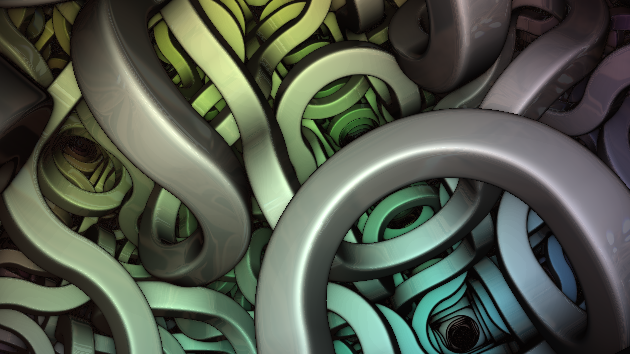
\includegraphics[scale=0.6]{img/logo.png}
    \end{textblock}

    \begin{textblock}{154} (28,135)
        \begin{picture}(150,2)
            \put(0,0){\color{bfhgrey}\rule{150mm}{2mm}}
        \end{picture}
    \end{textblock}
    \color{black}

    \begin{flushleft}
        \vspace*{120mm}
        \fontsize{26pt}{28pt}\selectfont
        \titel{}\\
        \vspace{3mm}
        \fontsize{14pt}{16pt}\selectfont
        \textbf{Projektarbeit 1} \\
        \vspace{6mm}

        \textbf{MTE7101} \\
        \vspace{3mm}

        \begin{textblock}{150} (28,215)
            \fontsize{10pt}{17pt}\selectfont
            \begin{tabbing}
            xxxxxxxxxxxxxxx   \= xxxxxxxxxxxxxxxxxxxxxxxxxxxxxxxxxxxxxxxxxxxxxxx \kill
            Studiengang:      \> Informatik                                         \\
            Autor:            \> Sven Osterwalder\protect\footnotemark[1]{}         \\
            Betreuer:         \> Prof.~Claude Fuhrer\protect\footnotemark[2]{} \\
            Datum:            \> \vhCurrentDate{}\\
            Version:          \> \vhCurrentVersion\\
            \end{tabbing}
        \end{textblock}
    \end{flushleft}
    \footnotetext[1]{sven.osterwalder@students.bfh.ch}
    \footnotetext[2]{claude.fuhrer@bfh.ch}

    \begin{textblock}{150} (28,280)
        \noindent
        \color{bfhgrey}\fontsize{9pt}{10pt}\selectfont
        Berner Fachhochschule | Haute école spécialisée bernoise | Bern University of Applied Sciences
        \color{black}\selectfont
    \end{textblock}

    \vfill
    
\includegraphics[height=\baselineskip]{img/by-sa}\\ \small{\sffamily{Licensed under the Creative Commons Attribution-ShareAlike 3.0 License}}

\end{titlepage}
          % activate for Titelseite mit Bild
\cleardoublepage{}
\phantomsection{}
% -*- coding: UTF-8 -*-
% vim: autoindent expandtab tabstop=4 sw=4 sts=4 filetype=tex
% chktex-file 27 - disable warning about missing include files

% Versionenkontrolle :
% -----------------------------------------------

\chapter*{}
\label{chap:versionen}

\begin{versionhistory}
    \vhEntry{0.1}{25.09.2015}{SO}{Initiale Erstellung des Dokumentes}
    \vhEntry{0.2}{27.09.2015}{SO}{Entwickeln einer initialen Struktur,
        Dokumentaufbau, Entwicklung Kapitel~\ref{chap:procedure}, Beschreibung von
        Ray Tracing in Kapitel~\ref{chap:theoretical_background}, Hinzufügen des
        Kapitels~\ref{chap:20_administrative}, Einführen von TODO-Notizen
    }
    \vhEntry{0.3}{29.09.2015}{SO}{Einführen von Meeting
        Minutes~\ref{chap:10_meeting_minutes}, Erweitern des
        Kapitels~\ref{chap:theoretical_background} um Belechtungsmodelle, Beschreiben von
        lokalen Beleuchtungsmodellen
    }
    \vhEntry{0.4}{04.10.2015}{SO}{Hinzufügen von Standards und
        Richtlinien~\ref{subsec:standards_guidelines}, Erweitern des
        Kapitels~\ref{chap:theoretical_background} um globale
        Belechtungsmodelle~\ref{subsec:global_illumination_models} sowie Ray
        Casting~\ref{subsec:ray_casting}, Entfernen der Schriftart `cmbright', Hinzufügen
        des Kapitels über (implizite) Oberflächen~\ref{sec:surfaces}
    }
    \vhEntry{0.5}{11.10.2015}{SO}{Neuordnung des
        Kapitels~\ref{chap:theoretical_background}: Hinzufügen des Kapitels über Ray
        Tracing~\ref{sec:ray_casting_tracing} sowie über Darstellung von impliziten
        Oberflächen~\ref{sec:description_implicit_surfaces}
    }
    \vhEntry{0.6}{14.10.2015}{SO}{Hinzufügen von TODO-Notizen, Anpassung der
        Textdarstellung in Formeln
    }
    \vhEntry{0.7}{16.10.2015}{SO}{Hinzufügen einer Illustration des
        Phong-Beleuchtungmodelles in Kapitel~\ref{subsec:local_illumination_models},
        Abarbeiten von TODO-Notizen in diversen Kapiteln, Erweitern des Kapitels über
        (implizite) Oberflächen~\ref{sec:surfaces}
    }
    \vhEntry{0.8}{17.10.2015}{SO}{Hinzufügen einer Illustration des Ray Tracing
        Algorithmus in Kapitel~\ref{subsec:global_illumination_models}
    }
    \vhEntry{0.9}{19.10.2015}{SO}{Beginn Kapitel über Rendering von impliziten
        Oberflächen~\ref{sec:rendering_implicit_surfaces}
    }
    \vhEntry{0.10}{21.10.2015}{SO}{Erweiterung Kapitel über Rendering von
        impliziten Oberflächen, Einführung Kapitel über die Umsetzung eines
        Prototypen~\ref{chap:prototype}
    }
    \vhEntry{0.11}{24.10.2015}{SO}{Umstrukturierung des Dokumentes, Anpassung
        der Dokumentvorlage, Nachführen der Versionshistorie, Ausführen der
        Meeting Minutes vom 18.10.2015, Erstellen der Vorlage für Meeting
        Minutes vom 25.10.2015
    }
    \vhEntry{0.12}{31.10.2015}{SO}{Nachführen der Versionshistorie, Ausführen der
        Meeting Minutes vom 25.10.2015, Erstellen der Vorlage für Meeting
        Minutes vom 02.11.2015, Erweiterung des
        Kapitels~\ref{chap:prototype}, Abarbeiten von TODO-Notizen
    }
    \vhEntry{0.13}{07.11.2015}{SO}{Ausführen der Meeting Minutes vom
        02.11.2015, Erweiterung des Kapitels~\ref{chap:prototype}
    }
    \vhEntry{0.14}{15.11.2015}{SO}{Erarbeiten des
        Kapitels~\ref{sec:rendering_implicit_surfaces_shadows},
        Erweiterung des Kapitels~\ref{chap:prototype} um weiche Schatten, 
        Erstellen und Hinzufügen von Bildmaterial zu Kapiteln~\ref{subsec:ray_marching}
        und~\ref{subsec:sphere_tracing}.
    }
    \vhEntry{0.15}{29.11.2015}{SO}{Komplette Überarbeitung des Bildmaterials zu
        Kapiteln~\ref{subsec:ray_marching} und~\ref{subsec:sphere_tracing}.
    }
    \vhEntry{0.16}{06.12.2015}{SO}{Nachführen von Meeting Minutes und der
        Versionierung. Überarbeiten des Zeitplanes, weiter Überarbeitung des
        Bildmaterials. Hinzufügen des Kapitels~\ref{sec:shading}, Hinzufügen
        einer Einleitung zu Kapitel~\ref{chap:theoretical_background}.
    }
\end{versionhistory}

\phantomsection{}
\cleardoubleemptypage{}
\listoftodos{}
\phantomsection{}
\cleardoubleemptypage{}
\setcounter{page}{1}
\cleardoublepage{}
\phantomsection{}
\addcontentsline{toc}{chapter}{Management Summary}
% -*- coding: UTF-8 -*-
% vim: autoindent expandtab tabstop=4 sw=4 sts=4 filetype=tex
% chktex-file 27

\chapter*{Management Summary}
\label{chap:managementSummary}

Lorem ipsum dolor sit amet, consectetur adipiscing elit. Phasellus scelerisque, leo sed iaculis ornare, mi leo semper urna, ac elementum libero est at risus. Donec eget aliquam urna. Lorem ipsum dolor sit amet, consectetur adipiscing elit. Nunc fermentum nunc sollicitudin leo porttitor volutpat. Duis ac enim lectus, quis malesuada lectus. Aenean vestibulum suscipit justo, in suscipit augue venenatis a. Donec interdum nibh ligula. Aliquam vitae dui a odio cursus interdum quis vitae mi. Phasellus ornare tortor fringilla velit accumsan quis tincidunt magna eleifend. Praesent nisl nibh, cursus in mattis ac, ultrices ac nulla. Nulla ante urna, aliquet eu tempus ut, feugiat id nisl. Nunc sit amet mauris vitae turpis scelerisque mattis et sed metus. Aliquam interdum congue odio, sed semper elit ullamcorper vitae. Morbi orci elit, feugiat vel hendrerit nec, sollicitudin non massa. Quisque lacus metus, vulputate id ullamcorper id, consequat eget orci.

\cleardoubleemptypage{}
%---------------------------------------------------------------------------

% Make sure Umlauts are getting displayed correctly.
\lstset{literate=%
    {Ö}{\textcolor{black}{\"O}}1
    {Ä}{{\"A}}1
    {Ü}{{\"U}}1
    {ß}{{\ss}}1
    {ü}{{\"u}}1
    {ä}{{\textcolor{black}{\"a}}}1
    {ö}{{\textcolor{black}{\"o}}}1
    {~}{{\textasciitilde}}1
    {?}{{\textcolor{black}{?}}}1
}
% Define a list style for Python programming language
\lstset{language=Python,
    basicstyle=\ttm,
    columns=fullflexible,
    commentstyle=\color{green},
    emphstyle=\ttb\color{red},
    frame=tb,
    identifierstyle=\color{black},
    keywordstyle=\ttb\color{blue},
    otherkeywords={self},
    % procnamekeys={def,class},
    showstringspaces=false,
    stringstyle=\color{green},
}

% Table of contents
%---------------------------------------------------------------------------
\tableofcontents
\cleardoublepage{}
%---------------------------------------------------------------------------

% Main part:
%---------------------------------------------------------------------------
\pagenumbering{arabic}
% -*- coding: UTF-8 -*-
% vim: autoindent expandtab tabstop=4 sw=4 sts=4 filetype=tex
% chktex-file 27 - disable warning about missing include files

\chapter{Einleitung}
\label{chap:10_introduction}

Seit dem Bestehen moderner Computer existiert auch die Computergrafik. Ziel der Computergrafik ist es unter Anderem den dreidimensionalen Raum auf eine zweidimensionale Fläche abzubilden, da die Ausgabe meist auf den zweidimensionalen Raum limitiert ist.

Dabei wird zwischen statischen Bildern und dynamischen Bildern unterschieden. Statische Bilder werden bei Bedarf dargestellt und ändern sich in der Regel nicht. Dynamische Bilder können sich hingegen ständig ändern und müssen --- bedingt durch das menschliche Auge --- mit 25 Bildern pro Sekunde ausgegeben werden. Es bestand bereits früh das Bestreben möglichst eine realistische Darstellung zu erhalten. Eine Darstellung also, die möglichst nahe an der menschlichen Wahrnehmung liegt.

Im Laufe der Zeit entstanden verschiedene Ansätze um eine solche Darstellung zu bieten. Ein Teilgebiet davon sind Beleuchtungsmodelle, welche die Beleuchtung einer Darstellung bzw.\ einer Szene berechnen. Dabei wird zwischen lokalen und globalen Beleuchtungsmodellen unterschieden.

Ein globales Beleuchtungsmodell ist Ray Tracing (zu deutsch Strahlenverfolgung), welches 1980 von Turner Whitted vorgestellt wurde wurde. Das Verfahren besticht durch seine Einfachheit und bietet dabei eine hohe Bildqualität mit perfekten Spiegelungen und Transparenzen. Mit entsprechenden Optimierungen ist das Verfahren auch relativ schnell.

Mit schnell ist dabei die Zeit gemeint, die benötigt wird um ein einzelnes Bild darzustellen. Möchte man jedoch eine Darstellung in Echtzeit erreichen, so war das Verfahren lange zu langsam.

Im Rahmen der Weiterentwicklung der Computer und vor allem durch die Weiterentwicklung der Grafikkarten (GPUs) ist Ray Tracing jedoch wieder in den Fokus der Darstellung von Szenen in Echtzeit gerückt.

Diese Projektarbeit stellt ein spezielles, auf Ray Tracing basierendes Verfahren zur Darstellung eines Bildes in Echtzeit vor: Das so Volume Ray Casting oder Sphere Tracing genannte Verfahren.

% -*- coding: UTF-8 -*-
% vim: autoindent expandtab tabstop=4 sw=4 sts=4 filetype=tex
% chktex-file 27 - disable warning about missing include files

\chapter{Administratives}
\label{chap:20_administrative}

\section{Beteiligte Personen}
\label{sec:involved_persons}

\section{Aufbau des Dokumentes}
\label{sec:document_structure}

\section{Ergebnisse}
\label{sec:deliverables}

% -*- coding: UTF-8 -*-
% vim: autoindent expandtab tabstop=4 sw=4 sts=4 filetype=tex
% chktex-file 27 - disable warning about missing include files

\chapter{Aufgabenstellung}
\label{chap:scope}

\section{Motivation}
\label{sec:motivation}

\todo[inline]{Describe motivation}

\subsection{Demoszene}
\label{subsec:demoscene}

\todo[inline]{Loose some words about demoscene! }

\section{Ziele und Abgrenzung}
\label{sec:objectives}

\todo[inline]{Describe objectives}

\subsection{Vorgängige Arbeiten}
\label{subsec:preliminaries}

\todo[inline]{Describe preliminaries}

\subsection{Neue Lerninhalte}
\label{subsec:new_learning_contents}

\todo[inline]{Describe new learning contents}

% -*- coding: UTF-8 -*-
% vim: autoindent expandtab tabstop=4 sw=4 sts=4 filetype=tex
% chktex-file 27 - disable warning about missing include files

\chapter{Vorgehen}
\label{chap:procedure}

\section{Arbeitsorganisation}
\label{sec:organization}

\subsection{Regelmässige Treffen}
\label{subsec:meetings}

Regelmässige Besprechungen mit dem Betreuer der Arbeit halfen die gesteckten Ziele zu erreichen und Fehlentwicklungen zu vermeiden. Der Betreuer unterstützte den Autor dabei mit Vorschlägen. Die Treffen fanden mindestens alle zwei Wochen statt, sie wurden in Form eines Protokolles festgehalten.

\section{Projekphasen}
\label{sec:project_schedule}

\subsection{Meilensteine}
\label{subsec:milestones}

Um bei der Arbeit ein möglichst strukturiertes Vorgehen einzuhalten, wurden folgende Projektphasen gewählt:
\begin{itemize}
    \item Projektstart
    \item Erarbeitung und Festhalten der Anforderungen
    \item Erarbeitung der theoretischen Grundlagen
    \item Erstellung der abschliessenden Dokumentation
\end{itemize}

Die Phasen der Erarbeitung der theoretischen Grundlagen sowie die Erstellung der abschliessenden Dokumentation liefen parallel ab.

\subsection{Zeitplan / Projektphasen}
\label{subsec:timeschedule}

\begin{figure}[H]
    \begin{ganttchart}[
        vgrid,
        x unit=0.7cm,
        bar/.append style={fill=bfhgrey!50},
    ]{1}{16}
        \gantttitle{2015}{14}
        \gantttitle{2016}{2} \\
        \gantttitlelist{1,...,16}{1} \\ % chktex 11: Disable "you should use \ldots to achieve.."
        \ganttbar{Projektstart}{1}{1} \\
        \ganttlinkedbar{Anforderungen}{2}{3} \ganttnewline{}
        \ganttbar{Erarbeitung theoretische Grundlagen}{2}{12} \\
        \ganttbar{Dokumentation}{1}{2} \ganttbar{}{1}{16} \\
        \ganttbar{Präsentation/Verteidigung vorbereiten}{15}{16}
    \end{ganttchart}
    \caption{Zeitplan; Der Titel stellt Jahreszahlen, der Untertitel Semesterwochen dar}
\end{figure}
\todo[inline]{Update schedule}
\todo[inline]{Add deadline for rough draft for end ov nov / beginning
    of dec}

\subsubsection{Projektstart}
\label{subsubsec:kick_off}
In der ersten Phase wurden die Meilensteine der Arbeit identifiziert und skizziert. Um Details der Aufgabe zu verstehen, wurde das notwendige Vorwissen über globale Beleuchtungsalgorithmen erarbeitet. Weiter wurde das Grundgerüst dieser Dokumentation erstellt.

\subsubsection{Anforderungen}
\label{ssubsec:requirements}
In dieser Phase wurde das Ziel dieser Projektarbeit festgelegt. Vom Ziel ausgehend wurden die dazu erforderlichen Projektphasen festgelegt.

\subsubsection{Erarbeitung theoretische Grundlagen}
\label{ssubsec:theoretical_background}
\todo[inline]{Describe theoretical background}

\subsubsection{Dokumentation}
\label{ssubsec:documentation}

Die vorliegende Arbeit entspricht der Dokumentation. Sie wurde während der gesamten Projektarbeit stetig erweitert und diente zur Reflexion von fertiggestellten Teilen.

\section{Technologien}
\label{sec:technologies}

\subsection{Tools und Software}
\label{subsec:tools_software}

\noindent\emph{Dokumentation}
\begin{description}
    \item[\LaTeX] Eine Makro-Sammlung für das \TeX-System. Wurde zur Erstellung
        dieser Dokumentation eingesetzt. Diese Dokumentation wurde mittels \LaTeX{} geschrieben.
    \item[Make] Build-Automations-Werkzeug, wurde zur Erstellung dieses Dokumentes eingesetzt.
    \item[zotero] Ein freies, quelloffenes Literaturverwaltungsprogramm zum Sammeln, Verwalten und Zitieren unterschiedlicher Online- und Offline-Quellen~\cite{wikipedia_foundation_zotero_2015}.
    \item[VIM] Vi IMproved. Ein freier, quelloffener Texteditor zur Textbearbeitung.
\end{description}

\noindent\emph{Arbeitsorganisation}
\begin{description}
    \item[Git] Freie Software zur verteilten Versionsverwaltung, wurde für die
        Entwicklung dieser Dokumentation verwendet. Die Projektarbeit findet sich
        unter~\href{https://www.github.com/sosterwalder/mte7101-project1}{GitHub}\footnote{\href{https://www.github.com/sosterwalder/mte7101-project1}{https://www.github.com/sosterwalder/mte7101-project1}}.
    \item[GitHub] Eine freie Hosting-Platform für Git mit Weboberfläche.
\end{description}

\subsection{Standards und Richtlinien}
\label{subsec:standards_guidelines}

\subsubsection{Pseudecode}
\label{ssubsec:standards_guidelines:psuedocode}

Da der Autor dieser Arbeit bedingt durch seine täglich Arbeit mit der Programmiersprache Python relativ bewandert ist, wird daher diese als Sprache zur Beschreibung von Pseudcode verwendet.
Dabei wird aber kein Augenmerk auf die formale Korrektheit, geschweige denn der Lauffähigkeit des Pseudocodes gelegt.

% -*- coding: UTF-8 -*-
% vim: autoindent expandtab tabstop=4 sw=4 sts=4 filetype=tex
% chktex-file 27 - disable warning about missing include files

\chapter{Theoretischer Hintergrund}
\label{chap:theoretical_background}

\section{Beleuchtungsmodelle}
\label{sec:illumination_models}

Sofern nicht anders vermerkt, basiert der folgende Abschnitt auf~\cite{whitted_improved_1980}[S. 343] sowie auf~\cite{hughes_computer_2013}.

Beleuchtungsmodelle beschreiben, wieviel Licht von einem sichtbaren Punkt einer Oberfläche zum Betrachter emitiert wird. In der Regel wird das Licht als Funktion in Abhängigkeit folgender Faktoren beschrieben:
\begin{itemize}
    \item Richtung der Lichtquelle \item Lichstärke
    \item Position des Betrachters
    \item Orientierung der Oberfläche
    \item Oberflächenbeschaffenheit
    \item Globale Umgebung
\end{itemize}

Es wird dabei zwischen lokalen und globalen Belechtungsmodellen unterschieden.

\subsection{Lokale Beleuchtungsmodelle}
\label{subsec:local_illumination_models}

Lokale Beleuchtungsmodelle aggregieren Daten von benachbarten, eben lokalen, Oberflächen. Diese Modelle sind in deren Umfang allerdings limitiert, da sie normalerweise nur Lichtquellen sowie die Orientierung einer Oberfläche einbeziehen. Sie ignorieren dabei aber die globale Umgebung, in welcher sich eine Oberfläche befindet.
Dies ist dadurch bedingt, dass die traditionell verwendeten Algorithmen zur Berechnung der Sichtbarkeit von Oberflächen, über keine globalen Daten verfügen.

Als Beispiel für ein lokales Beleuchtungsmodell dient das Phong-Beleuchtungsmodell, welches von Bui-Tong Phong entwickelt wurde.
Es beschreibt die reflektierte (Licht-) Intensität als Zusammensetzung aus der ambienten, der diffusen und der ideal spiegelnden Reflexion einer Oberfläche:
\begin{equation}
    I = I_{ambient} + I_{diffuse} + I_{specular}
\end{equation}
oder mathematisch ausgedrückt:
\begin{equation}
    I = I_a + k_d \displaystyle\sum_{j=1}^{ls} (\overrightarrow{N} \cdot \overrightarrow{L_j}) + k_s \displaystyle\sum_{j=1}^{ls} (\overrightarrow{N} \cdot \overrightarrow{L_j^`} )
\end{equation}
wobei gilt:
\begin{itemize}
    \item $I$:                      Die reflektierte (Licht-) Intensität
    \item $I_a$:                    Reflektion bedingt durch die Beleuchtung des Raumes
    \item $k_d$:                    Konstante für die diffuse Komponente des reflektierten Lichtes
    \item $\overrightarrow{N}$:     Einheitsnormale der Oberfläche
    \item $\overrightarrow{L_j}$:   Vektor in Richtung der $j$-ten Lichtquelle
    \item $k_s$:                    Koeffizient der spiegelenden Komponente
    \item $\overrightarrow{L_j^`}$: Vektor in der Hälfte zwischen dem Betrachter und der $j$-ten Lichtquelle
    \item $n$:                      Exponent, welcher von der Reflektion der Oberfläche abhängt
    \item $ls$:                     Anzahl Lichtquellen
\end{itemize}

\subsection{Globale Beleuchtungsmodelle}
\label{subsec:global_illumination_models}

Sofern nicht anders vermerkt, basiert der folgende Abschnitt auf~\cite{foley_computer_1996}[S. 775ff]

Globale Beleuchtungsmodelle beschreiben die reflektierte (Licht-) Intensität eines Punktes aufgrund direkter Lichteinstrahlung durch Lichtquellen sowie durch alles Licht, welches diesen Punkt nach Reflektion von bzw. Durchdringen der eigenen oder anderer Oberflächen erreicht.

Bei globalen Beleuchtungsmodellen unterscheidet man zwischen blickwinkelabhängigen Algorithmen, wie etwa Ray Tracing, und zwischen blickwinkelunabhängigen Algorithmen, wie etwa Photon Mapping.

Blickwinkelabhängige Algorithmen verwenden eine Diskretisierung~\todo{view plane} der sichtbaren Fläche um zu entscheiden, an welchen Punkten, in Blickrichtung des Betrachters, die Beleuchtungsberechnung durchgeführt werden soll. Blickwinkelunabhängige Algorithmen hingegen diskretisieren und verarbeiten die Umgebung um genügend Informationen für die Beleuchtungsberechnung zu haben. Dies erlaubt ihnen die Beleuchtungsberechnung an einem beliebigen Punkt aus einer beliebigen Blickrichtung.

Beide Arten von Algorithmen haben jedoch Vor- und Nachteile. So sind blickwinkelabhängige Algorithmen gut geeignet um Spiegelungen, basierend auf der Blickrichtung des Betrachtes, zu berechnen, eignen sich aber weniger um gleichbleibende diffuse Anteile über weiter Flächen eines Bildes zu berechnen. Bei blickwinkelabhängigen Algorithmen verhält es sich genau umgekehrt.

\subsubsection{Renderinggleichung}
\label{ssubsec:rendering_equation}

Die unter~\ref{subsec:global_illumination_models} genannten Verfahren versuchen auszudrücken, wie sich Licht von einem Punkt im Raum zu einem anderen bewegt. Dabei beschreiben sie die Intensität des Lichtes, ausgehend vom ersten Punkt zum zweiten Punkt. Zusätzlich wird die Intensität des Lichtes, ausgehend von allen anderen Punkten, welche den ersten Punkt erreichen, und zum zweiten Punkt emitiert werden, beschrieben.

James (Jim) Kajiya stellte 1986 die so genannte Renderinggleichung auf, welche genau dieses Verhalten beschreibt:
\begin{equation}
    I(x, x') = g(x, x')[\epsilon(x, x') + \int\limits_{s}\rho(x, x', x'')I(x', x'')dx'']
\end{equation}
wobei gilt:

\captionof{table}{Beschreibung der Komponenten der Renderinggleichung nach~\cite{kajiya_rendering_1986}[S. 143]}
\begin{tabular}{ l l }
    $ x', x' und x''   $: & Punkte in der Umgebung                                                                                                  \\
    $ I(x, x')         $: & Lichtintensität von Punkt $x'$ nach Punkt $x$                                                                           \\
    $ g(x, x')         $: & \parbox[t]{14cm}{Ein auf die Geometrie bezogener Term:                                                                  \\
                                 \hspace*{12mm} $0$:     \hspace*{6mm} $x$ und $x'$ verdecken sich                                                  \\
                                 \hspace*{12mm} $1/r^2$: \hspace*{1mm} $x$ und $x'$ sehen sich, wobei $r$ die Distanz zwischen $x$ und $x'$ ist}    \\
    $ \epsilon(x, x')  $: & Intensität des Lichtes, welches von $x'$ nach $x$ emitiert wird                                                         \\
    $ \rho(x, x', x'') $: & Intensität des Lichtes, welches von $x''$ durch die Oberfläche bei $x'$ nach $x$ gestreut wird                          \\
    $ \int\limits_{S}  $: & \parbox[t]{14cm}{Integral über die Vereinigung aller Flächen, daher $ S = \bigcup{S_{i}} $                              \\
                            Dies bedeutet, dass die Punkte $x$, $x'$ und $x''$ über alle Flächen aller Objekte der Szene ``streifen''.              \\
                            Wobei es sich bei $S_{0}$ um eine zusätzliche Fläche handelt, welche als Hintergrund verwendet wird.                    \\
                            $S_{0}$ ist dabei eine Hemisphäre, welche die gesamte Szene umspannt.}                                                  \\
\end{tabular}

\section{Ray Casting}
\label{sec:ray_casting}

Sofern nicht anders vermerkt, basiert der folgende Abschnitt auf~\cite{hughes_computer_2013}[Kapitel 15, S. 387ff].\\
\\
Um ein Bild möglichst realistisch darzustellen muss berechnet werden, wieviel Licht zu jedem Pixel der sichtbaren Bildfläche (also dem Betrachter) transportiert wird. Da Photonen die Energie des Lichtes transportieren, muss man also das physikalische Verhalten dieser simulieren. Es ist allerdings nicht möglich \textit{alle} Photonen zu simulieren, da der Aufwand schlicht zu gross wäre. Daher macht es Sinn nur einige Photonen (exemplarisch) zu betrachten und dann eine Abschätzung des gesamten Lichtes vorzunehmen.\\
\\
Bei \textbf{Ray Casting} handlt es sich grundsätzlich um eine Strategie zur Simulation, wieviel Licht anhand eines (Licht-) Strahles zu der sichtbaren Bildfläche (also dem Betrachter) transportiert wird.

\begin{figure}[H]
    \centering \rotatebox{0}{\scalebox{0.3}[0.3]{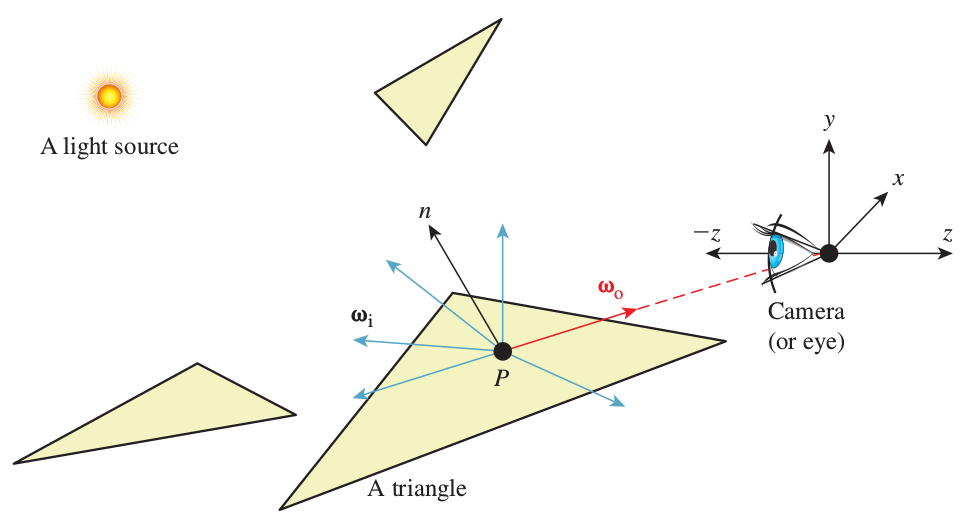
\includegraphics{img/ray_tracing_01.png}}}
    \caption{Punkt $P$ auf einer Oberfläche eines Dreieckes, welcher für die Kamera bzw.\ den Betrachter sichtbar ist.
        Der Betrachter nimmt dabei das Licht, welches aus verschiedenen Richtungen $\omega_{i}$ kommt, über den Punkt $P$ in Richtung $\omega_{0}$ wahr.\label{fig:ray_casting:basics}\protect\footnotemark}
\end{figure}
\footnotetext{Darstellung von~\cite{hughes_computer_2013}[Kapitel 15, Seite 389, Abbildung 15.1]}

Wie in Abbildung~\ref{fig:ray_casting:basics} ersichtlich, gelangt Licht aus vielen Richtungen durch den Punkt $P$ zu dem Betrachter. Dies beinhaltet auch die Möglichkeit, dass
Licht nicht nur von einer Lichtquelle aus, sondern von vielen Lichtquellen aus via $P$ zum Betrachter gelangt. Weiter ist es möglich, dass Licht zuvor an anderen Punkten gestreut
und/oder gespiegelt und erst dann via $P$ zum Betrachter gelangte.\\
\\
Dies führt zu den folgenden Schlussfolgerungen:
\begin{itemize}
    \item Es müssen alle möglichen Richtungen, aus denen Licht kommen könnte, an Punkt $P$ untersucht werden.
    \item Da, bedingt durch technische Limitierungen, nur diskretes Abtasten möglich ist, müssen die Richtungen auf eine endliche Anzahl beschränkt werden, was zu Abtastfehlern führen kann.
\end{itemize}
Um die Abtastfehler zu minieren, können die Richtungen des Abtasten anhand der Lichtquellen priorisiert werden.

\newpage{}

Ein möglicher Algorithmus, wie solch ein Verfahren umgesetzt werden kann, findet sich in~\ref{fig:ray_casting:high_level}.

\begin{python}[caption={Eine abstrakte Umsetzung des Ray Castings.\protect\footnotemark},label={fig:ray_casting:high_level}]
def ray_cast():
    # "pixels" is a list of all pixels of the image plane
    for pixel in pixels:
        # Save all intersections for given pixel
        intersections = []

        # Returns the ray passing through the given
        # pixel from the eye
        ray           = ray_at_pixel(pixel)

        # "scene_triangles" is a list of all triangles
        # coming from meshes contained in the scene to render
        for triangle in scene_triangles:
            p   = intersect(ray, triangle)
            sum = 0

            for light in incoming_lights_at_p:
                sum = sum + l.value
            end

            if is_smallest_intersection(p, intersections):
                pixel = sum
            intersections.append(p)
\end{python}
\footnotetext{Algorithmus in Pseudocode gemäss~\cite{hughes_computer_2013}[Kapitel 15, Seite 391, Auflistung 15.2]}

\newpage{}

\section{Ray Tracing}
\label{sec:ray_tracing}

\todo[inline]{Since illumination returned to the viewer is deter-
mined by a tree of ``rays,'' a ray tracing algorithm is
ideally suited to this model. In an obvious approach to
ray tracing, light rays emanating from a source are traced
through their paths until they strike the viewer. Since
only a few will reach the viewer, this approach is waste-
ful. In a second approach suggested by Appel [1] and
used successfully by MAGI [14], rays are traced in the
opposite direction---from the viewer to the objects in the
scene, as illustrated in Figure 4.
Unlike previous ray tracing algorithms, the visibility
calculations do not end when the nearest intersection of
a ray with objects in the scene is found. Instead, each
visible intersection of a ray with a surface produces more
rays in the /\~ direction, the /5 direction, and in the
direction of each light source. The intersection process is
repeated for each ray until none of the new rays intersects
any object.}

\section{Darstellung impliziter Oberflächen}
\label{sec:implicit_surfaces}

\todo[inline]{Describe implicit surfaces}

% -*- coding: UTF-8 -*-
% vim: autoindent expandtab tabstop=4 sw=4 sts=4 filetype=tex
% chktex-file 27 - disable warning about missing include files

\chapter{Oberflächen}
\label{chap:surfaces}

% -*- coding: UTF-8 -*-
% vim: autoindent expandtab tabstop=4 sw=4 sts=4 filetype=tex
% chktex-file 27 - disable warning about missing include files

\section{Oberflächen}
\label{sec:surfaces}

Sofern nicht anders vermerkt, basiert der folgende Abschnitt
auf~\cite{division_introduction_1996}[S. 1 ff].\\
\\
Um in Computergrafiken überhaupt etwas darstellen zu können, muss erst einmal
definiert werden, was dargestellt werden soll. Häufig orientiert sich die
Computergrafik dabei an der realen Welt.  In der realen Welt haben Oberlächen
von Objekten häufig keine starken Übergänge (Kanten) sondern sind eher von
glatter Natur~\cite{foley_computer_1996}[S. 471].\\
\\
Die Darstellung von Kurven und Oberflächen führt zu zwei Fällen: Modellierung
von bestehenden Objekten und Modellierung von Grund auf.\\
\\
Zur Modellierung von Oberflächen werden hauptsächlich zwei Techniken verwendet:
Parametrische Modellierung und implizite Modellierung.\\
\\
Bei der parametrsichen Darstellung wird eine Oberfläche überlicherweise als
eine Menge von Punkten definiert, so zum Beispiel:

\begin{gather}\label{eq:surface_parametric}
    \bm{p}(s, t) = (x(s, t), y(s, t), z(s, t))
\end{gather}

Die Einheitskugel mit Radius 1, würde beispielsweise wie folgt mittels der
parametrischen Darstellung beschrieben:


\begin{gather}\label{eq:unit_sphere_parametric}
    \bm{unitsphere}(s, t) = (x^{2}(s, t), y^{2}(s, t), z^{2}(s, t)) - 1^{2}
\end{gather}
\todo[inline]{Check if correct}

Bei der impliziten Darstellung wird eine Oberfläche überlicherweise als Kontur
einer Funktion mit Wert 0 definiert, so zum Beispiel:

\begin{gather}\label{eq:surface_implicit}
    f(\bm{p}) = f(x, y, z) = 0
\end{gather}

Daher am Beispiel der Einheitskugel:

\begin{gather}\label{eq:unit_sphere_implicit}
    f(\bm{unitsphere}) = f(x^{2}, y^{2}, z^{2}) - 1 = 0
\end{gather}
\todo[inline]{Check if correct}

Die parametrische Darstellung bringt Vorteile wie die Unabhängigkeit von einem
Koordinatensystem oder eine effiziente Berechnung von Punkten auf einer
Oberfläche. Die implizite Darstellung erlaubt hingegen eine grössere
Einflussnahme aus mathematischer Sicht und ist daher sehr nützlich für
Operationen wie Biegung, Vermischung, Schnitte (Intersektion) oder Bool'sche
Operationen.

\subsection{Implizite Oberflächen}
\label{subsec:implicit_surfaces}

Wie in Gleichung~\ref{eq:surface_parametric} beschrieben, ist eine implizite
Oberfläche gemäss~\cite{hart_ray_1993}[S. 1] als Funktion $ f(\bm{x}) =
\mathbb{R}^{3} \to \mathbb{R} $ definiert.  Es wird also jedem Punkt einer
Menge $ \bm{p} \in \mathbb{R}^{3} $ ein skalarer Wert $ s \in \mathbb{R} $
zugewiesen. Dabei besteht die Oberfläche aus der Punktemenge $ \bm{x} \equiv
(x, y, z) \in \mathbb{R}^{3} $.\\
\\
Angenommen $ \bm{A} $ ist ein geschlossener Festkörper, welcher durch die
Funktion $f$ beschrieben wird, dann kann gemäss~\cite{hart_ray_1993} Folgendes
angenommen werden:

\begin{align} \label{eq:surface_implicit_condition}
    x \in \overset{\circ}{\bm{A}} \Leftrightarrow f(\bm{x}) &< 0 \\
    x \in \partial \bm{A}         \Leftrightarrow f(\bm{x}) &= 0 \\
    x \in \mathbb{R}^{3} - \bm{A} \Leftrightarrow f(\bm{x}) &> 0
\end{align}

Dies bedeutet, dass sich ein Punkt $\bm{x}$:
\begin{itemize}
    \item $\overset{\circ}{\bm{A}}$, genau dann \textit{innerhalb} des Körpers
        $\bm{A}$ befindet, wenn die implizite Funktion $f(\bm{x})$ \textit{negativ}
        ist
    \item $\partial{\bm{A}}$, genau dann \textit{auf der Oberfläche} des
        Körpers $\bm{A}$ befindet, wenn die implizite Funktion $f(\bm{x})$
        \textit{0} ist
    \item $\mathbb{R}^{3} - \bm{A}$, \textit{nicht in oder auf} dem Körper
        $\bm{A}$ befindet, wenn die implizite Funktion $f(\bm{x})$ \textit{positiv}
        ist
\end{itemize}

Dies gilt, da es sich bei $ \bm{x} $ um eine Punktemenge mit topologischer
Struktur handelt.\\
\\
Gemäss~\cite{division_introduction_1996} finden hauptsächlich drei Methoden
Anwendung zur Beschreibung impliziter Oberflächen: algebraische Oberflächen,
Blobby-Objekte sowie die funktionale Repräsentation.~\cite{hart_sphere_1994}
gibt jedoch an, dass die gebräuchlichste Form von impliziten Oberflächen die
algebraischen Oberflächen sind. Diese werden implizit durch polynomiale
Funktionen definiert.\\

\subsubsection{Algebraische und geometrische implizite Oberflächen}
\label{ssubsec:implicit_surfaces_algebraic_geometric}

Ein Beispiel für eine algebraische Oberfläche ist die Beschreibung der
Einheitskugel anhand einer impliziten algebraischen Gleichung zweiten Grades:

\begin{gather} \label{eq:surface_immplicit_algebraic}
    x^{2} + y^{2} + z^{2} - 1 = 0
\end{gather}

Wobei es sich bei dem letzten Parameter um den Radius $r$ handelt, welcher ---
bedingt durch die Einheitskugel --- den Wert 1 hat.

Wie~\cite{division_introduction_1996} schreibt, handelt es sich bei impliziten
Oberflächen, welche durch eine polynomiale Funktion zweiten Grades beschrieben
werden, um quadrische implizite Oberflächen.

\cite{hart_sphere_1994} gibt weiter an, dass --- unter Nuztung einer Metrik ---
die Einheitskugel durch die implizite Gleichung

\begin{gather} \label{eq:surface_immplicit_geometric}
    \|\bm{x}\| - 1 = 0
\end{gather}

beschrieben werden kann, was unter Anwendung der allgemeinen
Form~\ref{eq:surface_implicit} einer impliziten
Gleichung~\ref{eq:surface_implicit} zu folgender Gleichung führt:

\begin{gather}\label{eq:surface_implicit_sphere}
    f(\bm{x}) = \|\bm{x}\| - 1
\end{gather}


Dabei ist $\|\bm{x}\|$ als euklidische Metrik definiert und entspricht ${(x^{2} + y^{2} + z^{2})}^{1 \over 2}$.\\
\\
Die Gleichung~\ref{eq:surface_immplicit_algebraic} gibt die algebraische
Distanz zurück, Gleichung~\ref{eq:surface_immplicit_geometric} gibt die
geometrische Distanz zurück.\\

\subsubsection{Distanzfunktionen}
\label{ssubsec:distance_functions}

Gemäss~\cite{hart_sphere_1994} wird die geometrische Darstellung von
quadrischen Oberflächen bevorzugt, da deren Parameter unabhängig von
Koordinaten sind, sie robuster und intuitiver sind. Es handelt sich dabei um
eine \textbf{Distanzfunktion}.\\
\\
Wie anfangs erwähnt, definiert~\cite{hart_sphere_1994} die allgemeine Form zur
Beschreibung bzw. Darstellung von impliziter Oberflächen als Zuweisung von
Punkten zu einem skalaren Wert: $ f : \mathbb{R}^{n} \to \mathbb{R} $.\\
\\
Unter Anwendung der unter~\ref{eq:surface_implicit_condition} definierten
Bedingungen kann geschlossen werden, dass eine Menge von Punkten $A$ existiert,
welche Teil von $\mathbb{R}^{n}$, also $A \subset \mathbb{R}^{n}$ ist. Dies heisst, dass alle Punkte in $A$ die folgende Bedingung erfüllen:

\begin{gather}
    A = \{ x : f(x) \leq 0 \}
\end{gather}

\cite{hart_sphere_1994} liefert zwei Definition, welche der Beschreibung von Distanzfunktionen dienen:

\theoremstyle{definition}
\begin{definition}{\label{theo:point_to_set_distance}
    \textit{Point-to-set distance}}\\
    Die Distanz eines Punktes zu einer Menge von Punkten definiert die Distanz
    eines Punktes $ \bm{x} \in \mathbb{R}^{3} $ zu einer Menge von Punkten $A
    \subset \mathbb{R}^{3}$ als Distanz von $\bm{x}$ zum nähesten Punkt in $A$:

    \begin{gather}
        d(\bm{x}, \bm{A}) = \min_{\substack{\bm{y} \in \bm{A}}}(\|\bm{x} - \bm{y}\|)
    \end{gather}
\end{definition}

\theoremstyle{definition}
\begin{definition}{\label{theo:signed_distnace_bound}
    \textit{Signed distance bound}}\\ 
    Eine Funktion $ f : \mathbb{R}^{3} \to \mathbb{R} $ ist eine
    vorzeichenabhängige Obergrenze ihrer impliziten Oberfläche $ f^{-1}(0)$,
    wenn gilt:

    \begin{gather}\label{eq:signed_distnace_bound}
        |f(\bm{x})| \leq d(\bm{x}, f^{-1}(0))
    \end{gather}
\end{definition}

Wenn die Gleichung~\ref{eq:signed_distnace_bound} für eine Funktion $f$ gilt,
dann ist $f$ eine \textit{vorzeichenabhängige Distanzfunktion (signed distance
    function)}.

\subsubsection{Distanzfelder (distance fields)}
\label{ssubsec:distance_fields}

\todo[inline]{Introduce distance fields?}

Sofern nicht anders vermerkt, basiert der folgende Abschnitt
auf~\cite{jones_3d_2006}.

Bei einem Distanzfeld handelt es sich um eine Repräsentation respektive eine
Datenstruktur, bei welcher von jedem Punkt aus die geringste Distanz zu
einem beliebigen Objekt der Domäne bekannt ist.

Zusätzlich zu der Distanz können aus einem Distanzfeld andere Parameter
wie beispielswiese die Richtung einer Oberfläche abgeleitet werden.

Handelt es sich bei einem Distanzfeld um ein vorzeichenbehaftetes
Distanzfeld, so kann bei jedem Punkt bestimmt werden, ob sich dieser
innerhalb, ausserhalb oder genau auf einem Objekt befindet. Dies verhält
sich analog zu Abschnitt~\ref{subsec:implicit_surfaces}.

Distanzfelder bilden somit die Grundlage der Algorithmen zur Darstellung
von impliziten Oberflächen. Siehe dazu auch
Kapitel~\ref{sec:rendering_implicit_surfaces}. Die unter
Abschnitt~\ref{ssubsec:distance_functions} genannte~\textit{Point-to-set
    distance}-Funktion  liefert bereits die näheste Distanz zu einer
Menge von Punkten und somit auch zu Objekten auseghend von einem Punkt
der Domäne.

\begin{figure}[H]
    \centering
    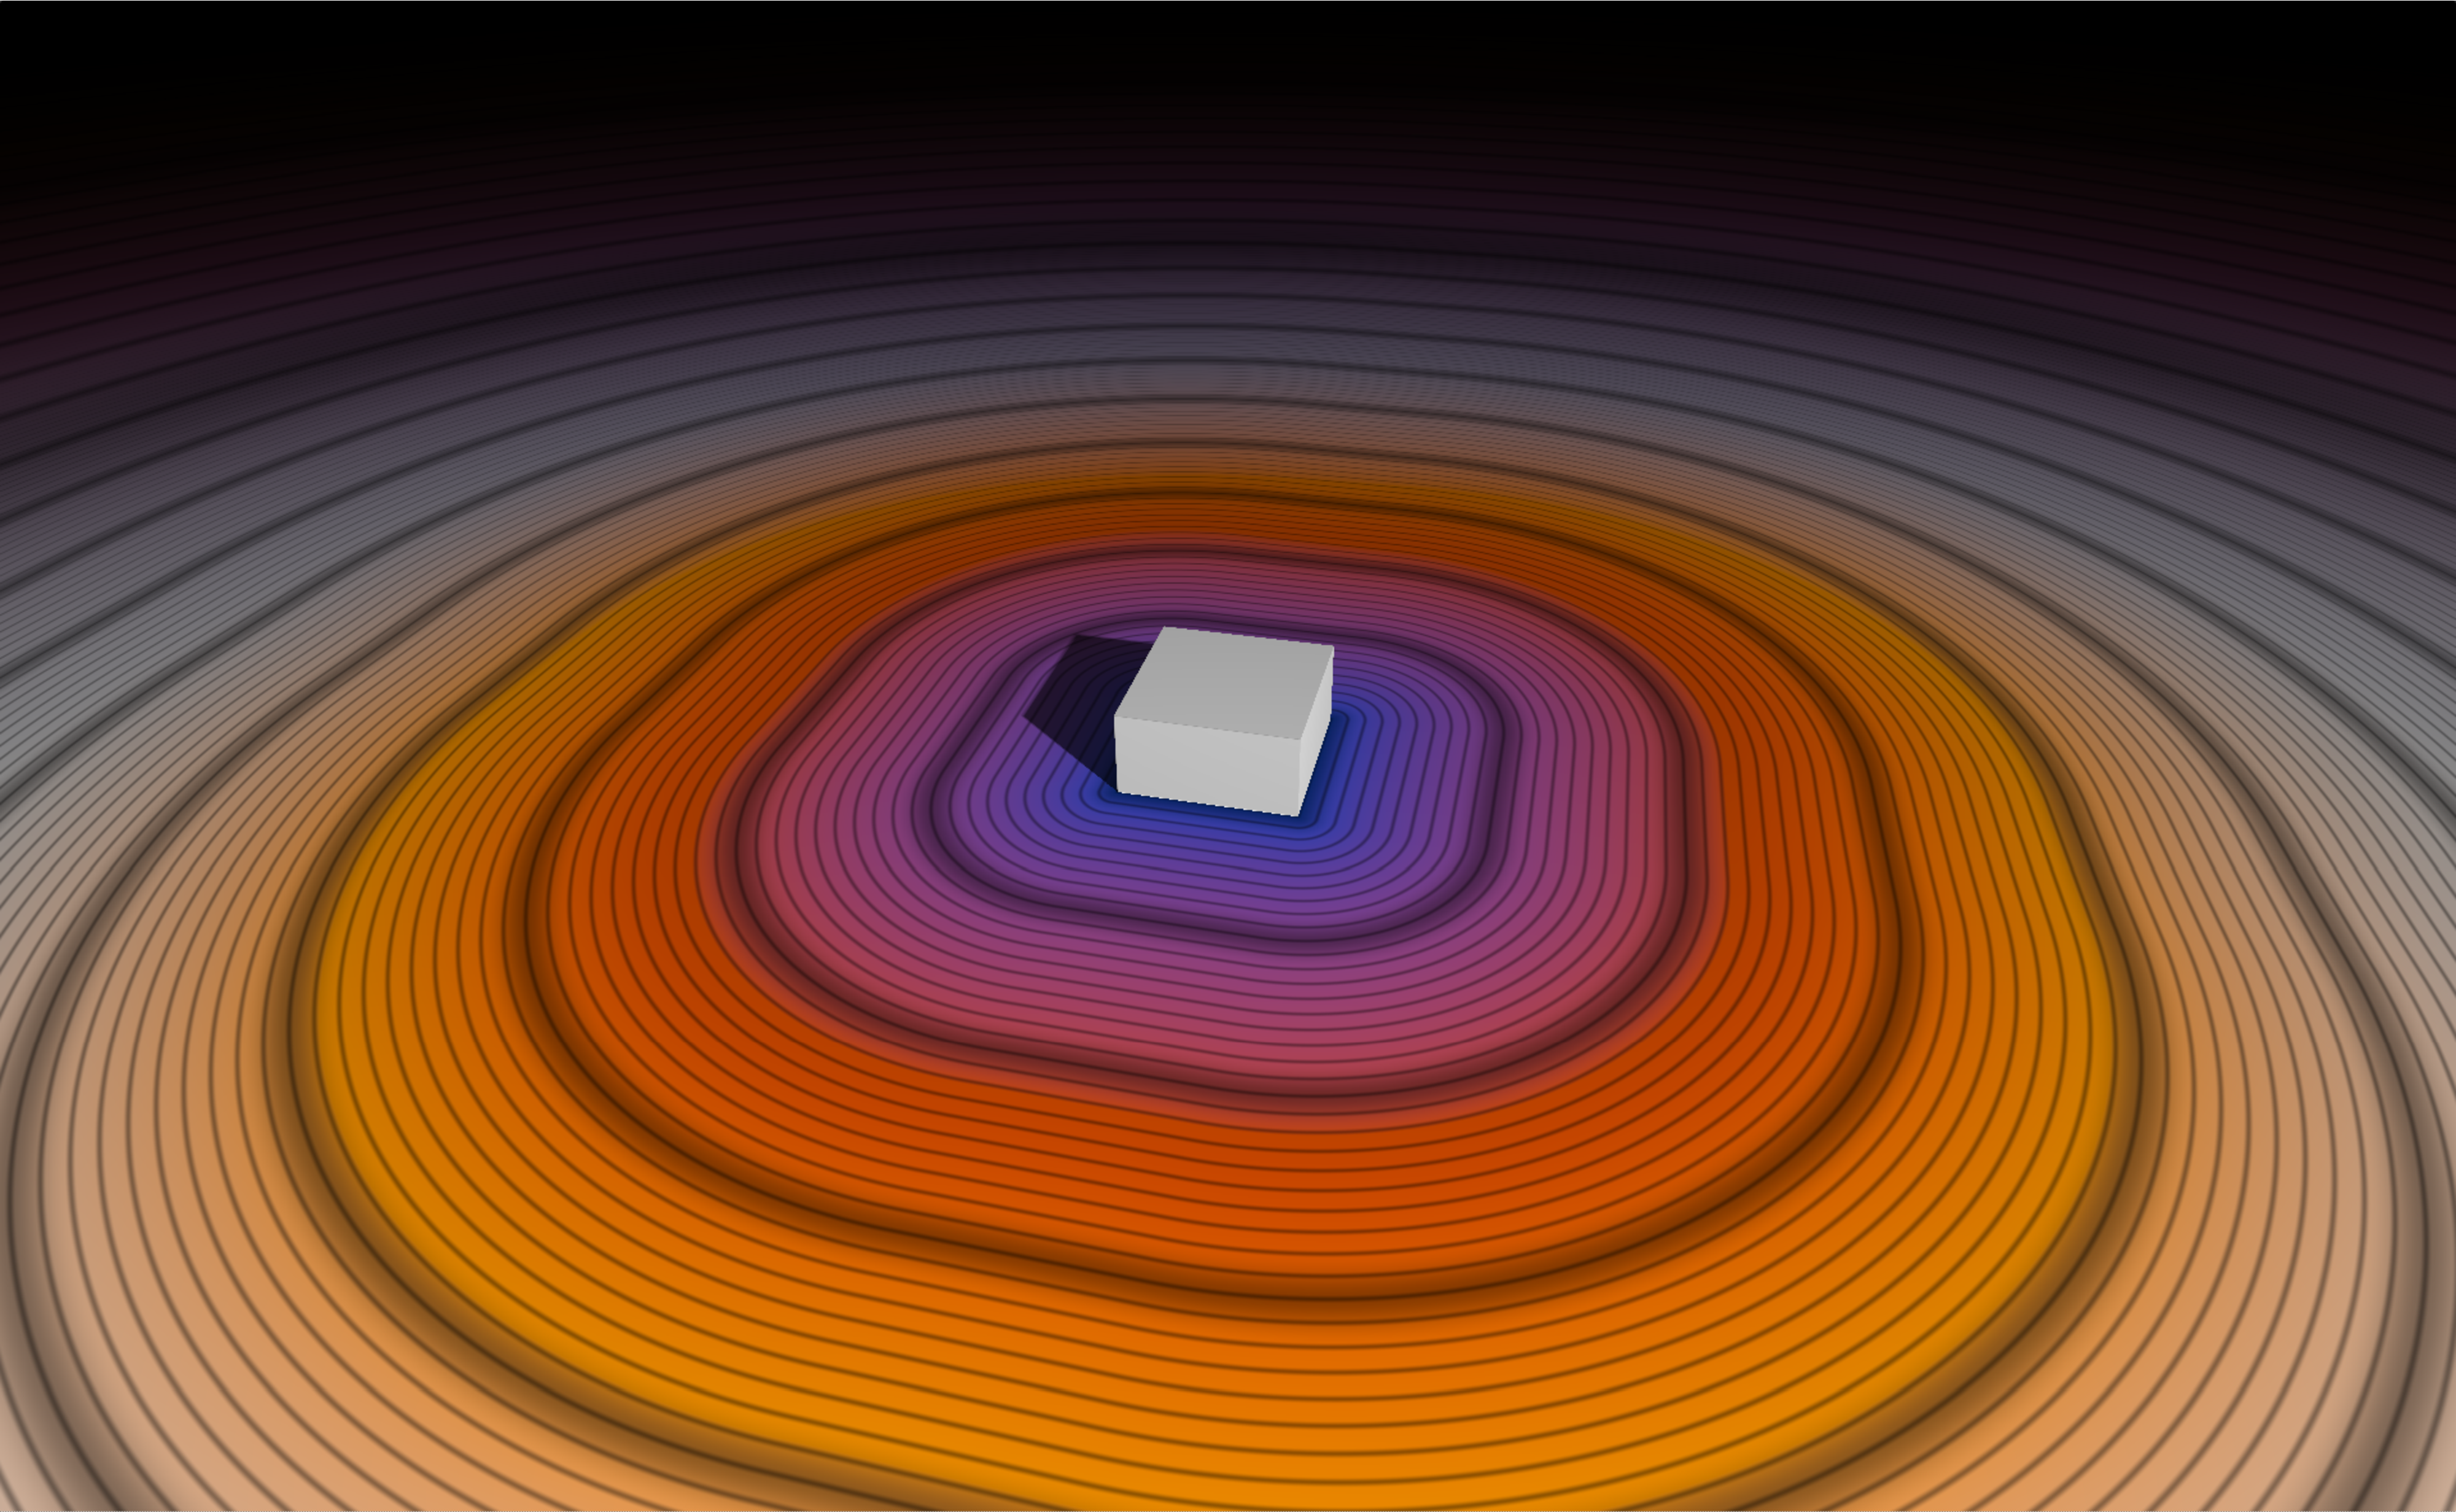
\includegraphics[width=1.0\textwidth]{img/distance_field.pdf}
    \caption{Darstellung des Dinstanzfeldes einer dreidimensionalen
        Szene anhand Farbwerten\protect\footnotemark}\label{
        fig:distance_field_illustration}
\end{figure}
\footnotetext{Eigene Darstellung}

% -*- coding: UTF-8 -*-
% vim: autoindent expandtab tabstop=4 sw=4 sts=4 filetype=tex
% chktex-file 27 - disable warning about missing include files

\section{Darstellung von impliziten Oberflächen}
\label{sec:description_implicit_surfaces}

Wie~\cite{hart_sphere_1994}[S. 1] angibt, existieren verschiedene Möglichkeiten
zur Darstellung (zum Rendering) von impliziten Oberflächen. So wandeln
indirekte Methoden implizite Oberflächen in Polygonmodelle um, was die Nuztung
bestehender Techniken und Hardware zur Darstellung von polygonalen Modellen
erlaubt. Obwohl die Umwandlung der impliziten Oberflächen mit gängigen Systemen
zur Darstellung problemlos dargestellt werden kann, ist die Umwandlung jedoch nicht
in jedem Fall gegeben und kann zu nicht zusammenhängenden Flächen oder einer
Verminderung des Detailgrades führen.\\
\\
Eine andere Methode zur Darstellung von impliziten Oberflächen ist das
unter~\ref{sec:ray_tracing} vorgestellte Ray Tracing Verfahren.

Ein (Licht-) Strahl wird dabei parametrisch als

\begin{gather}\label{eq:ray_param}
    r(t) = r_{0} + t \cdot r_{d}
\end{gather}

beschrieben. Der Strahl startet dabei bei Punkt $r_{0}$ in Richtung des
Einheitsvektors $r_{d}$, wobei $t$ die zurückgelegte Distanz des Strahles ist.
Dabei ist $r(t)$ der Punkt im Raum, welchen der Strahl nach dem Zurücklegen der
Distanz $t$ --- ausgehend von seinem Ursprung $r_{0}$ --- erreicht.\\
\\
Um nun die Schnittpunkte eines Strahles mit einer impliziten Oberfläche zu finden, wird die Gleichung des Lichtstrahles $r$ (\ref{eq:ray_param}) in die Funktion einer impliziten Oberfläche $f$ (\ref{eq:surface_implicit}) eingesetzt. Wobei $r : \mathbb{R} \to \mathbb{R}^{3}$ und $f : \mathbb{R}^{3} \to \mathbb{R}$. Dies ergibt die zusammengesetzte Funktion $F = f \circ r$ wobei $F : \mathbb{R} \to \mathbb{R}$.\\
\\
Die Lösungen dieser Gleichung sind alle Distanzen $t$, welche ein gegebener Strahl zurücklegt und welche die folgende Bedingung erfüllen:

\begin{gather}\label{eq:ray_param_cond}
    F(t) = f \circ r = f(r(t)) = 0
\end{gather}

Um die Gleichung~\ref{eq:ray_param_cond} zu lösen, können numerische Verfahren
zur Nullstellensuche angewendet werden, wobei die Verfahren vom Typ der
Funktion $F(t)$ abhängig sind. Bei polynomialen Funktionen bis zum vierten Grad
existieren analytische Lösungen, für eine beliebige Funktion muss jedoch ein
generisches, robustes Verfahren zur Nullstellensuche verwendet werden. Dies
bedingt jedoch meist, dass mehr Informationen über die Funktion zur Verfügung
stehen, was beispielsweise durch Ableiten dieser gelöst werden kann.\\
\\
Die erwähnten Verfahren zur Nullstellensuche haben jedoch häufig den Nachteil,
dass sie mehrere Schnittpunkte eines Strahles mit einer impliziten Oberfläche
liefern. Um diese Problematik zu umgehen, wird nur der kleinste Wert von $t$
berücksichtigt. Die Ray Marching und Sphere Tracing Algorithmen gehen hier
sogar noch einen Schritt weiter, in dem sie nur die kleinste positive
Nullstelle der Gleichung~\ref{eq:ray_param_cond} betrachten.

\subsection{Ray Marching}
\label{subsec:ray_marching}

~\cite{perlin_hypertexture_1989} schlagen eine Abtastung des Strahles mit fixen
Abständen $\Delta \mu$ vor:

\begin{gather}
    x = x_{\mu_{0}} + k \cdot \Delta x_{\mu}
\end{gather}

wobei $k = 0,1,2,\dots$ und $\mu_{0} + k \Delta \mu \leq \mu_{1}$.\\
\\
Auf die parametrische Darstellung eines (Licht-) Strahles,
Gleichung~\ref{eq:ray_param_cond}, angwendet:

\begin{gather}
    r(k) = r_{0} + \Delta t \cdot k \cdot r_{d}
\end{gather}

wobei $\Delta t$ die Grösse der Abstände und $k = 0,1,2,\dots$ die Nummer der
Schritte darstellt. Wie~\cite{hart_ray_1989} schreiben, bildet das Abtasten des
(Licht-) Strahles mit fixen Abständen die Basis für gewisse Verfahren des
volumetrischen Renderings.\\
\\
Ein möglicher Algorithmus, wie solch ein Verfahren umgesetzt werden kann,
findet sich in~\ref{fig:ray_marching}.

\begin{lstlisting}[language=Python,caption={Eine abstrakte Umsetzung des Ray
        Marchings\protect\footnotemark.},label={fig:ray_marching},captionpos=b,emph={ray_march}]
def ray_march():
    step         = 0
    intersection = 0
    max_steps    = 10

    while step < max_steps:
        intersection = test_intersection(k)

        if intersection <= 0:
            # An intersection has happened
            #   intersection <  0: ray is inside surface
            #   intersection == 0: ray is excatly on surface
            return ray_travel_distance(step)

        step = step + 1

    # When we reach this step, after max_steps, no intersection
    # has happened, so distance is 0
    return 0
\end{lstlisting}
\footnotetext{Algorithmus in Pseudocode
    gemäss~\cite{perlin_hypertexture_1989}[S. 259, Abschnitt 3.1]}

Dabei ist jedoch zu beachten, dass der Abstand zur Abtastung eines Strahles
$\Delta t$ so gering als möglich sein sollte um eine Punktemeng bzw.\ ein
Objekt --- definiert durch implizite Oberflächen --- $A$ möglichst gut
abschätzen zu können. Ist der gewählte Abstand zu gross gewählt, so findet ggf.
eine Abtastung weit im Inneren des Objektes statt und somit geht Präzision
verloren.  Es ist auch möglich dass der erste eigentliche Punkt gar nicht
abgetastet wird und erst der zweite abgetastete Punkt das Objekt ``erkennt''.

\begin{figure}[H]
    \caption{Illustration des Ray Marching Verfahrens und dessen
    Problemen.\protect\footnotemark}\label{fig:ray_marching_problems}
    \centering
    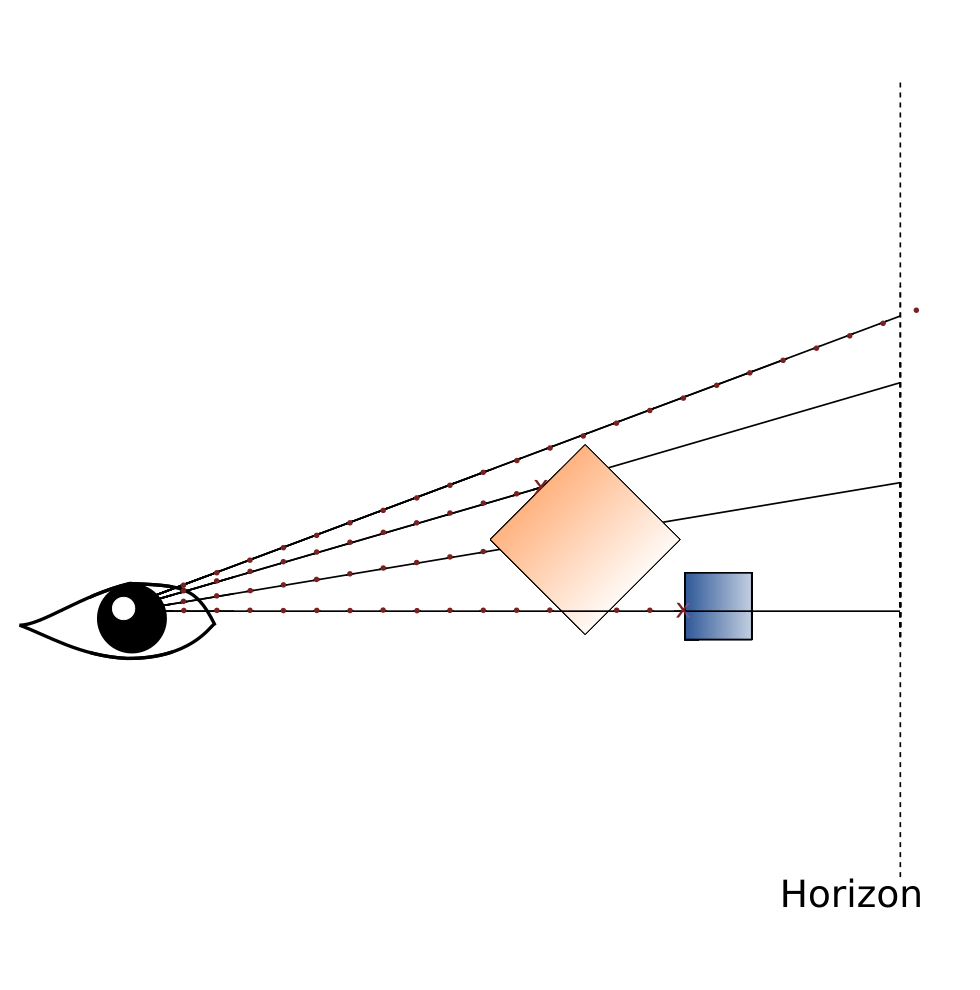
\includegraphics[width=0.5\textwidth]{img/ray_marching_problems.png}
\end{figure}
\footnotetext{Eigene Darstellung mittels Geogebra.}

Die Abbildung~\ref{fig:ray_marching_problems} veranschaulicht diese
Problematiken. Zu sehen sind vier Primärstrahlen, \textit{e},
\textit{f}, \textit{g} und \textit{h},  sowie zwei Objekte,
\textit{poly1} und \textit{poly2}.

Bei den Strahlen \textit{e} und \textit{g} handelt es sich um
``normale'' Fälle: Der Strahl \textit{e} geht komplett an den Objekten
vorbei, das Ray Marching wird also nach erreichen der maximalen Distanz
\textit{d\textsubscript{max}} abgebrochen, der Strahl \textit{g} trifft
das Objekt \textit{poly1} nach 6 Schritten.

Bei den Strahlen \textit{f} und \textit{h} handelt es sich um
Spezialfälle: Der Strahl \textit{f} trifft das Objekt \textit{poly1}
nicht, obwohl der Strahl durch das Objekt hindurch geht. Dies geschieht
aufgrund der gewählten Distanz zum Abtasten der Strahlen ($\Delta t$).
Der Strahl \textit{h} trifft das Objekt \textit{poly2}, obwohl er
eigentlich das Objekt \textit{poly1} treffen müsste. Das getroffene
Objekt \textit{poly2} dürfte so gar nicht zu sehen sein. Dieser Fehler
tritt wiederum aufgrund der gewählten Distanz zur Abtastung der Strahlen
($\Delta t$) auf.

\cite{hart_sphere_1994} weist darauf hin, dass Ray Marching durch den möglichst
geringen Abstand zwischen den Abtastungen entsprechend langsam und paralleles
Abtasten praktisch unumgänglich ist. In der von~\cite{hart_sphere_1994}
vorgestellten Technik des Sphere Tracings ist der Abstand zwischen den
Abtastungen nicht konstant sondern variiert in Abhängigkeit der Geometrie.

\subsection{Sphere Tracing}
\label{subsec:sphere_tracing}

Das von~\cite{hart_sphere_1994} vorgestellte Sphere Tracing Verfahren ist ein
Ray Tracing (\ref{sec:ray_tracing}) Verfahren für implizite Oberflächen. Es
handelt sich nach wie vor um Ray Marching (\ref{subsec:ray_marching}), die
Distanz der Schritte zum Abtastens  eines (Licht-) Strahles wird jedoch
aufgrund einer Distanzfunktion (\ref{ssubsec:distance_functions}) bestimmt.\\
\\
\cite{hart_sphere_1994} verweist auf den Term \textit{``unbounding volumes''},
welcher in~\cite{hart_ray_1989} eingeführt wurde. ``Unbounding volumes'' (zu
Deutsch etwa ``negativer Hüllkörper'') wird genutzt um Sphere Tracing zu
beschreiben und darzustellen. Der Term steht im Gegensatz zu dem gängigen
Konzept des Hüllkörpers (``bounding volumes'') --- ein Volumen, welches einen
Körper umschliesst. Ein ``negativer Hüllkörper'' (``unbounding volume'')
umschliesst also eine Fläche im Raum, welche den Körper \textit{nicht}
beinhaltet.\\
\\
Man möchte für einen abzutastenden Punkt im Raum ein Volumen finden, wessen
Zentrum im abzutastenden Punkt liegt. Ist der Abstand des Punktes zum nähesten
Punkt der Oberfläche eines Objektes bekannt, kann dieser Abstand als Radius
einer Kugel angenommen werden. Diese Kugel dient als negativer Hüllkörper
(``unbounding Volume'') und ist \textit{garantiert nicht} Teil des Objektes und
schneidet dieses auch nicht (ist also nicht $\overset{\circ}{\bm{A}}$) --- nur
der äusserste Punkt des Abstandes (also des Radius der Kugel) liegt genau auf
der Oberfläche des Objektes ($\partial \bm{A}$). Der Radius solch einer Kugel
wird durch Evaluation der Distanzfunktion eines abzutastenden Punktes im Raum
bestimmt.\\
\\
Gemäss~\cite{hart_sphere_1994} kommt daher auch der Name Sphere Tracing: Die
Schnittpunkte eines (Licht-) Strahles werden durch eine Folge von negativen
Hüllkörpern (``unbounding volumes'') --- bzw.\ in diesem Fall Kugeln
(``unbounding spheres'') --- beschrieben.\\
\\
Da~\cite{hart_ray_1989} die Darstellung von Fraktale im dreidimensionalen Raum
beschreibt, wird dort von einer Abschätzung der Distanz gesprochen. Dies ist
dadurch bedingt, dass die Distanz für Fraktale nicht effizient berechnet werden
kann. Betrachtet man jedoch die Darstellung von  ``regulären'' Objekten, wie zum
Beispiel eine Kugel, kann der zur Oberfläche am nähesten gelegene Punkt von
einem beliebigen Punkt derselben Domäne exakt berechnet werden. Dies ist durch
die implizite Gleichung~\ref{eq:surface_implicit_sphere} gegeben.\\
\\
Gemäss~\cite{hart_ray_1989} verläuft die Strahlenverfolgung bei dem Sphere
Tracing Verfahren wie folgt. Ein Strahl wird vom Betrachter (Auge bzw.
Lochkamera) durch die Bildebene zu einem Objekt geschossen. Dabei wird beim
initialen Augangspunkt der Radius eines negativen Hüllkörpers in Form einer
Kugel --- so wie oben beschrieben --- berechnet. Dies ist die Distanz, welcher
der Strahl in einem ersten Schritt effektiv zurücklegen wird. Bei jedem
Schnittpunkt der Kugel mit dem Strahl wird dasselbe Verfahren wiederholt. Dies
geschieht so lange, bis schliesslich der Strahl durch einen Schnittpunkt mit
einem Radius auf die Oberfläche des Objektes trifft. Ein weiteres
Abbruchkriterium ist eine definierte maximale Distanz eines Strahles. Ist diese
erreicht und der Strahl erreicht die Oberfläche des Objektes nicht --- weil der
Strahl das Objekt nicht schneidet oder das Objekt zu weit weg ist ---, wird
abgebrochen. Somit ist auch ersichtlich, dass Sphere Tracing nicht die
unter~\ref{subsec:ray_marching} genannten Problematiken aufweist.


\begin{figure}[H]
    \caption{Illustration des Sphere Tracing Verfahrens.\protect\footnotemark}\label{fig:sphere_tracing_1}
    \centering
    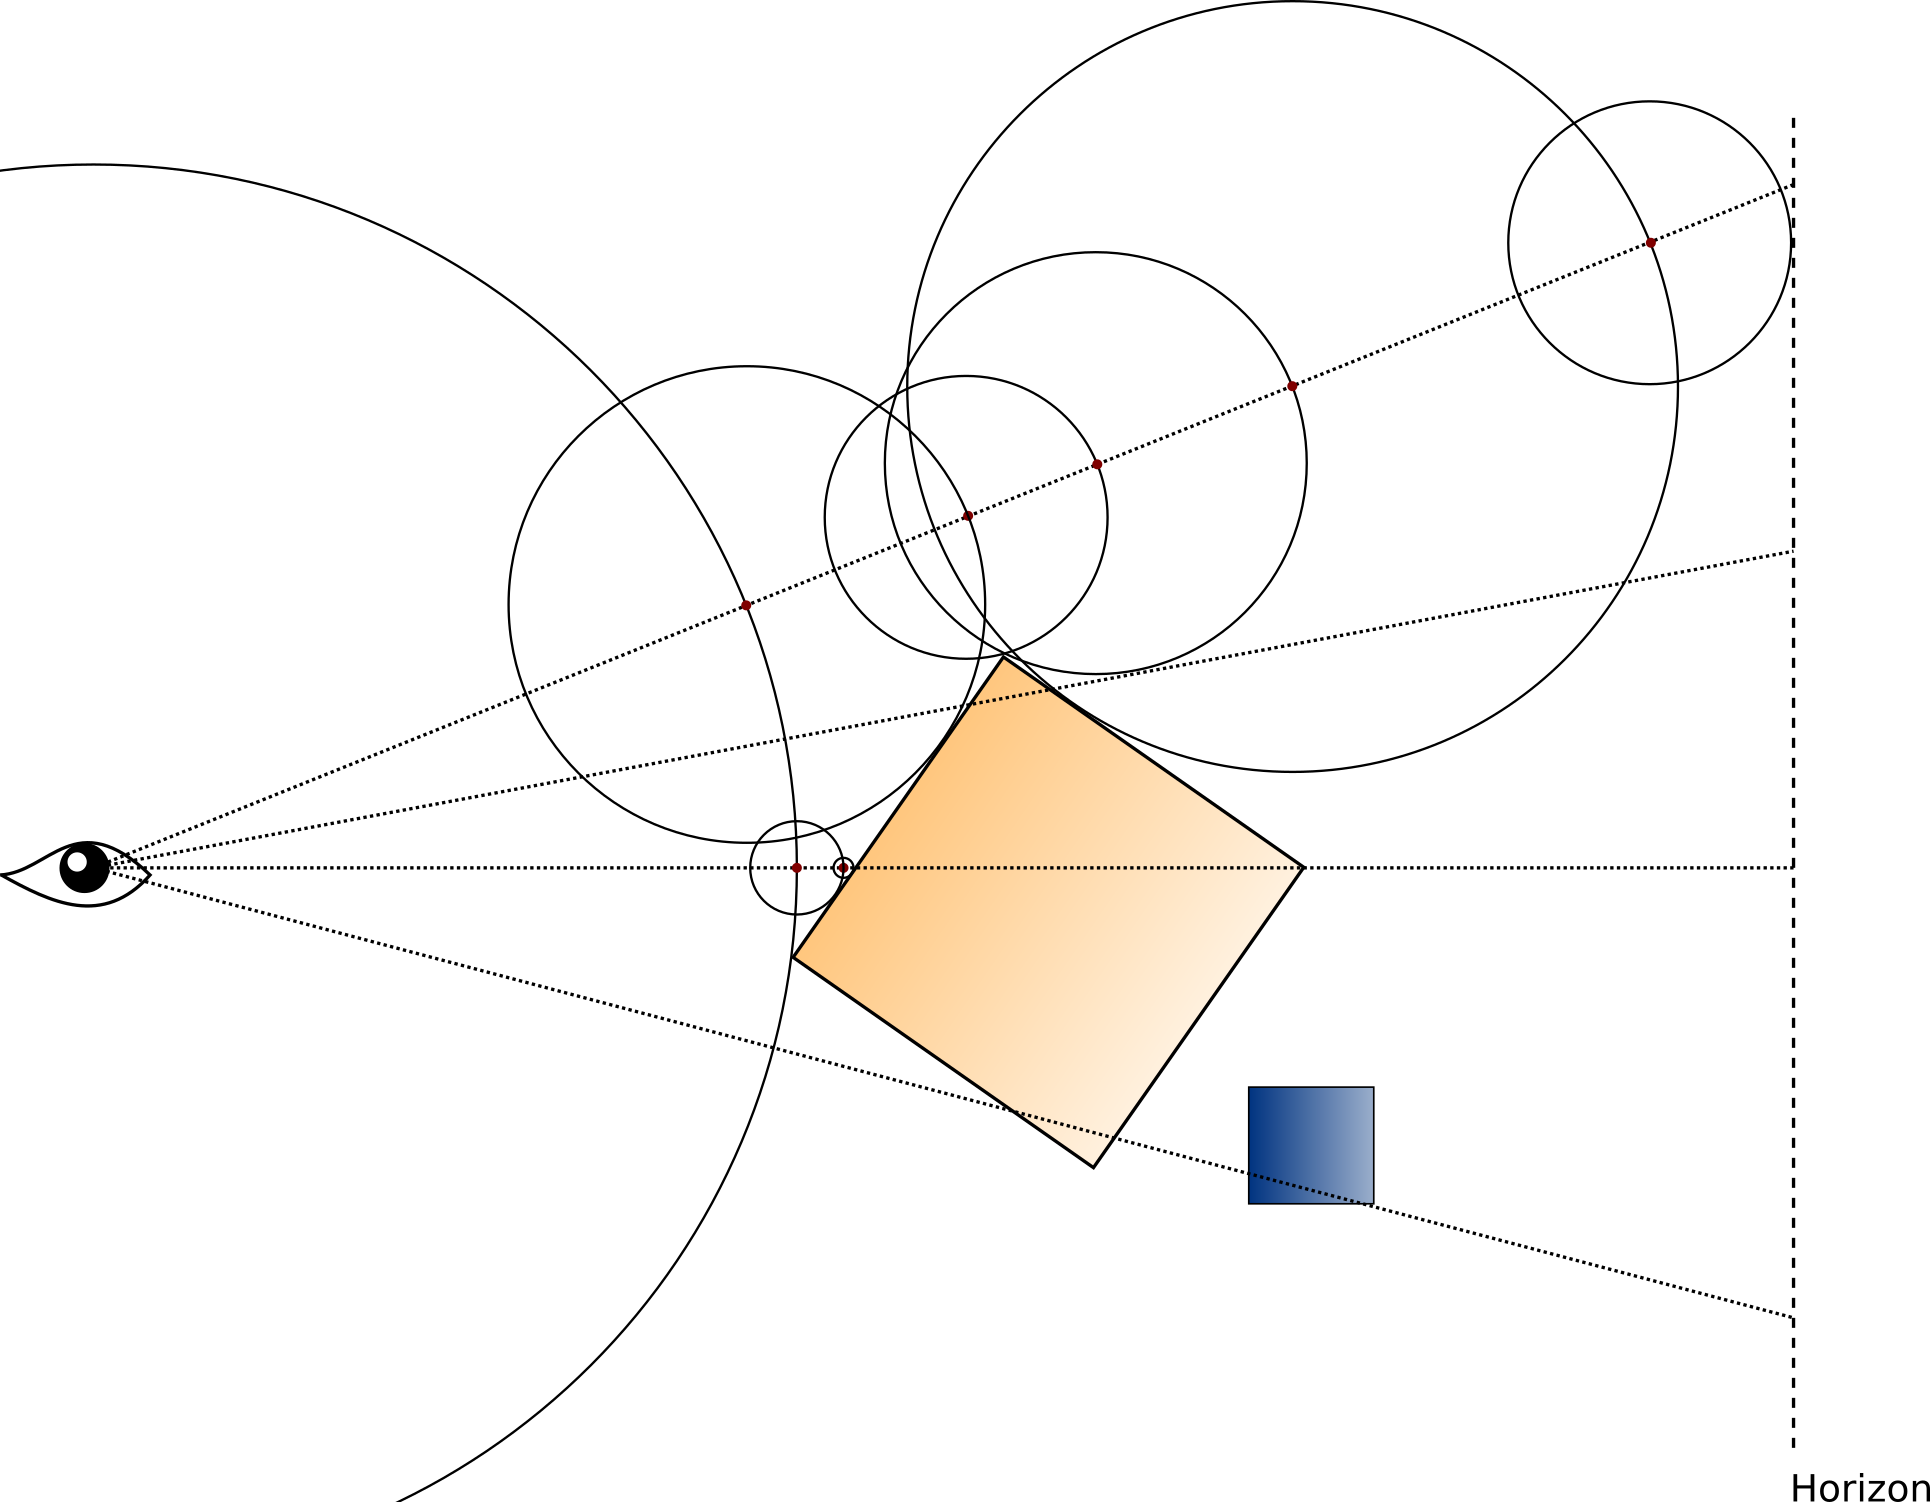
\includegraphics[width=1.0\textwidth]{img/sphere_tracing_principle.png}
\end{figure}
\footnotetext{Eigene Darstellung mittels Inkscape.}
\begin{figure}[H]
    \caption{Illustration des Sphere Tracing Verfahrens, Nahaufnahme.\protect\footnotemark}\label{fig:sphere_tracing_2}
    \centering
    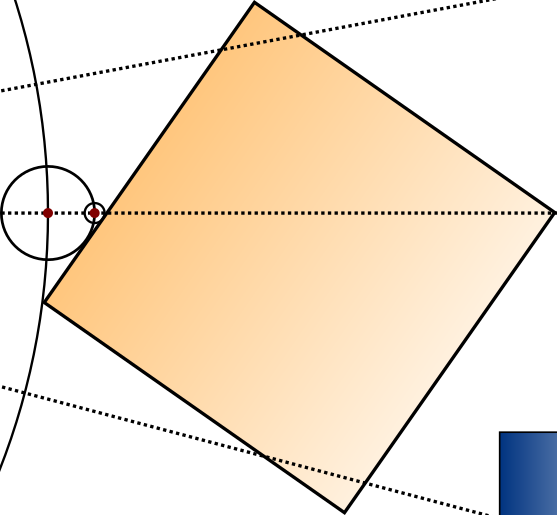
\includegraphics[width=0.5\textwidth]{img/sphere_tracing_principle_1.png}
\end{figure}
\footnotetext{Eigene Darstellung mittels Inkscape.}
\begin{table}[H]
    \centering
    \caption{INSERT CAPTION HERE\protect\footnotemark}\label{table:sphere_tracing_3}
    \begin{tabular}{p{0.3\textwidth}p{0.3\textwidth}p{0.3\textwidth}}
        \toprule
            \textbf{kShadow: \textit{8.0}} &
            \textbf{kShadow: \textit{16.0}}   &
            \textbf{kShadow: \textit{32.0}}   \\
        \cmidrule(r){1-1}\cmidrule(lr){2-2}\cmidrule(l){3-3}
            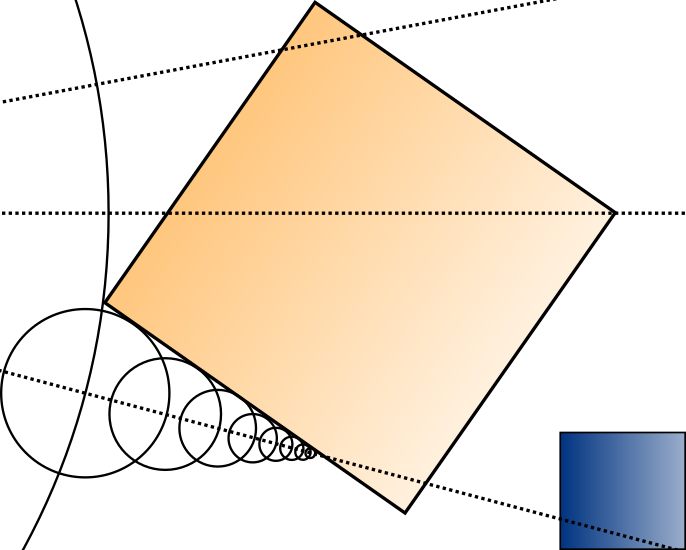
\includegraphics[width=0.3\textwidth]{img/sphere_tracing_principle_3_0.png} \newline &
            
\includegraphics[width=0.3\textwidth]{img/sphere_tracing_principle_3_1.png} \newline &
            \includegraphics[width=0.3\textwidth]{img/sphere_tracing_principle_3_2.png} \newline \\
        \bottomrule
    \end{tabular}
\end{table}
\footnotetext{Eigene Darstellung mittels Inkscape.}

Ausgehend von der parametrischen Beschreibung eines (Licht-) Strahles
(Gleichung~\ref{eq:ray_param}), beschreibt~\cite{hart_sphere_1994} die Richtung
$r_{d}$ eines Strahles als Einheitsvektor:

\begin{gather}
    r_{d} = \frac{p_{x, y} - r_{0}}{|p_{x, y} - r_{0}|}
\end{gather}

wobei $r_{0}$ der Ursprung eines Strahles und $p_{x, y}$ ein Punkt der Bildebene ist.\\
\\
Um nun den Schnittpunkt eines Strahles $r_{d}$ mit der Oberfläche eines
Objektes zu finden, muss die Gleichung $F(t)$ (\ref{eq:ray_param_cond}) gelöst
werden. Dabei ist --- wie oben definiert --- die Funktion $f(x)$ nun eine
Distanzfunktion wie die geometrische Distanzfunktion zur Beschreibung einer
Kugel (Gleichung~\ref{eq:surface_immplicit_geometric}).\\
\\
Evaluiert man nun die Gleichung $F(t)$ unter Anwendung der eben beschriebenen
Strahlenverfolgung, findet man so die erste positive Nullstelle der Gleichung
$F(t)$. Diese Nullstelle ist die Grenze der Folge von negativen Hüllkörpern
(``unbounding spheres''), welche durch die rekursive Gleichung:

\begin{gather}
    t_{i+1} = t_{i} + F(t_{i})
\end{gather}

definiert ist. Der Ursprungspunkt ist dabei als $t_{0}$ definiert. Diese Folge
konvergiert genau dann --- und nur dann --, wenn der Strahl auf die implizite
Oberfläche eines Objkektes trifft. Diese Folge bildet den Kern des Algorithmus
zur Darstellung von geometrisch definierten, impliziten Oberflächen.

\begin{lstlisting}[language=Python,caption={Eine abstrakte Umsetzung des Sphere
        Tracings\protect\footnotemark.},label={alg:sphere_tracing},captionpos=b,emph={sphere_trace}]
def sphere_trace():
    ray_distance          = 0
    estimated_distance    = 0
    max_distance          = 9001
    convergence_precision = 0.000001

    while ray_distance < max_distance:
        # sd_sphere is a signed distance function defining the implicit surface
        # cast_ray defines the ray equation given the current travelled /
        # marched distance of the ray
        estimated_distance = sd_sphere(cast_ray(ray_distance))

        if estimated_distance < convergence_precision:
            # the estimated distance is already smaller than the desired
            # precision of the convergence, so return the distance the ray has
            # travelled as we have an intersection
            return ray_distance

        ray_distance = ray_distance + estimated_distance

    # When we reach this point, there was no intersection between the ray and a
    # implicit surface, so simply return 0
    return 0
\end{lstlisting}
\footnotetext{Algorithmus in Pseudocode gemäss~\cite{hart_sphere_1994}[S. 531,
    Fig. 1]}

\subsection{Operationen für implizite Oberflächen}
\label{subsec:implicit_surfaces_ops}

Um mit impliziten Oberflächen nicht nur einfache Objekte, wie zum Beispiel eine
Kugel darzustellen, möchte man diese auch transformieren können.

Wie~\cite{hart_sphere_1994}[S. 543] beschreibt, werden implizite Oberflächen
durch die Invertierung des Raumes, in welchem sich die Oberfläche befindet,
transformiert. Der Raum, in dem sich eine implizite Oberfläche befindet, ist
die Domäne der impliziten Funktion der Oberfläche.

Sei $T(\bm{x})$ eine Transformation und $f(\bm{x})$ eine Distanzfunktion,
welche eine implizite Oberfläche definiert. Somit ist die transfomierte
implizite Oberfläche:

\begin{gather}
    f(T^{-1}(\bm{x})) = 0
\end{gather}

Bei Transformationen handelt es sich um vorzeichenabhängige Distanzfunktion
(signed distance functions).

Es werden dabei folgende Arten von Transformationen unterschieden:
\begin{itemize}
    \item Distanzoperationen, wie zum Beispiel Vereinigung, Subtraktion oder Intersektion
    \item Domänenoperationen, wie zum Beispiel Wiederholung, Rotation, Translation und Skalierung
    \item Distanzdeformationen, wie zum Beispiel Versatz (displacement) und Vermengung/Vermischung (blend)
    \item Domänendeformationen, wie zum Beispiel ``Verderung'' (twist) und Biegung (bend)
\end{itemize}

\subsubsection{Isometrien}
\label{ssubsec:implicit_surfaces_ops_isometries}

Nicht alle Transformationen erhalten dabei die Distanz, welche die
Distanzfunktion der transformieren Oberfläche zurückgeben würde. In solch einem
Falle ist die zurückgegebene Distanz nicht die Distanz eines beliebigen Punktes
im Raum zu dem ihm nähesten Punkt einer impliziten Oberfläche.

Transformationen, welche hingegen distanzerhaltend sind,
bezeichnet~\cite{hart_sphere_1994} als~\textit{Isometrien}. Dazu zählen
Rotationen, Translationen aber auch Reflektionen.

Ist $\bm{I}$ eine Isometrie, dann benötigt die zurückgegebene Distanz der
Distanzfunktion $f(\bm{x})$ \textit{keine Anpassung}.

\begin{gather}
    d(\bm{x}, \bm{I} \circ f^{-1}(0)) = d(\bm{I}^{-1}(\bm{x}), f^{-1}(0))
\end{gather}

Wobei $\bm{I}$ eine Isometrie und $f^{-1}(0)$ eine implizite Oberfläche ist.

\subsubsection{Uniforme Skalierung}
\label{ssubsec:implicit_surfaces_ops_scaling}

Eine Skalierung ist \textit{nicht} distanzerhaltend, daher \textit{erhält} sie die Distanz, welche die
Distanzfunktion der skalierten Oberfläche zurückgeben würde, \textit{nicht}.
Somit muss die zurückgegebene Distanz entsprechend angepasst werden.

\cite{hart_sphere_1994} gibt die uniforme Skalierung als Transformation $\bm{S(x)}$  der Form:

\begin{gather}
    \bm{S(x)} = s \cdot \bm{x}
\end{gather}

an, wobei $s$ der Skalierungsfaktor ist. Die Invertierung der Skalierung ist gegeben als:

\begin{gather}
    \bm{S^{-1}(x)} = {1 \over s} \cdot \bm{x}
\end{gather}

Somit ist die Distanz zu der skalierten impliziten Oberfläche:

\begin{gather}
    d(\bm{x}, \bm{S}(f^{-1}(0))) = s \cdot d(\bm{S}^{-1}(\bm{x}), f^{-1}(0))
\end{gather}

Dabei wird die von der Distanzfunktion der skalierten impliziten Oberfläche
zurückgegebene Distanz mit dem Skalierungsfaktor $s$ multipliziert, was die
eigentliche Distanzinformation erhält und die Skalierung somit isometrisch
macht.

\subsubsection{``Verdrehung'' (Twist)}
\label{ssubsec:implicit_surfaces_ops_twist}

Gemäss~\cite{hart_sphere_1994}[S. 543] werden bei der ``Verdrehung'' (Twist)
einer impliziten Oberfläche zwei Achsen (z.B. $x$ und $y$) anhand einer
linearen Funktion $a(\cdot)$ in Abhängigkeit der dritten Achse (z.B. $z$)
rotiert:

\begin{gather}
    twist(\bm{x}) = \begin{pmatrix} 
        x \cdot \cos{a(z)} - y \cdot \sin{a(z)},\\
        x \cdot \sin{a(z)} + y \cdot \cos{a(z)},\\
        z
    \end{pmatrix}
\end{gather}

\subsubsection{Vereinigung}
\label{ssubsec:implicit_surfaces_ops_union}

Die Vereinigung zweier impliziter Oberflächen $A$ und $B$ wird
von~\cite{hart_sphere_1994} als minimale Distanz der jeweiligen
vorzeichenabhängigen  Distanzfunktion $f_{A}$ respektive $f_{B}$ definiert:

\begin{gather}
    d(\bm{x}, A \cup B) = \min(f_{A}(\bm{x}), f_{B}(\bm{x}))
\end{gather}

wobei $\bm{x}$ den abzutastenden Punkt im Raum darstellt.

Wie~\citeauthor{hart_sphere_1994} schreibt, ist die Distanz zu einer Liste von
impliziten Oberflächen die kleinste Distanz der jeweiligen Distanzfunktion.
Somit erlaubt es die Vereinigung --- neben der eigentlichen Vereinigung von
Objekten --- mehrere implizite Oberflächen zu kombinieren, ohne dass diese
miteinander in Kontakt stehen müssen. So kann beispielsweise eine komplexe
Szene modelliert werden.

\subsubsection{Subtraktion}
\label{ssubsec:implicit_surfaces_ops_subtraction}

Um die Operation der Subtraktion zu definieren, wird die Distanz zum Komplement
eines Objektes $\bm{A}$ verwendet. Dabei wird die Eigenschaft der
Vorzeichenabhängigkeit von vorzeichenabhängigen Distanzfunktionen genutzt:

\begin{gather}
    d(\bm{x}, \mathbb{R}^{3} \setminus A) = -f_{A}(\bm{x})
\end{gather}

Somit kann die Subtraktion zweier impliziter Oberflächen $A$ und $B$
gemäss~\cite{hart_sphere_1994} als Intersektion eines Objektes $A$ mit der
Subtraktion des Raumes bzw.\ der Domäne mit einem Objekt $B$ angesehen werden,
daher folgt:

\begin{align}
    d(\bm{x}, A - B) &= A \cap (\mathbb{R}^{3} \setminus B) \\
                     &\geq \max(f_{A}(\bm{x}), -f_{B}(\bm{x}))
\end{align}

wobei $\bm{x}$ den abzutastenden Punkt im Raum darstellt.

\subsubsection{Intersektion}
\label{ssubsec:implicit_surfaces_ops_intersection}

Die Intersektion zweier impliziter Oberflächen $A$ und $B$ wird
von~\cite{hart_sphere_1994} als minimale Distanz der jeweiligen
vorzeichenabhängigen  Distanzfunktion $f_{A}$ respektive $f_{B}$ definiert:

\begin{gather}
    d(\bm{x}, A \cap B) \geq \max(f_{A}(\bm{x}), f_{B}(\bm{x}))
\end{gather}

wobei $\bm{x}$ den abzutastenden Punkt im Raum darstellt.

\subsection{Primitive}
\label{subsec:implicit_surfaces_primitives}

\cite{hart_sphere_1994} führt in seinem Paper~\todo{Use another word?} einige
(geometrische) Primitve auf, welche nachfolgende erläutert werden.

\subsubsection{Ebene}
\label{ssubsec:implicit_surfaces_primitives_plane}

Die vorzeichenbehaftete Distanz zu einer Ebene $P$ mit einer Einheitsnormalen
$\bm{n}$, welche sich mit dem Punkt $\bm{n} \cdot r$ schneidet ist wie folgt
definiert:

\begin{gather}
    d(\bm{x}, P) = \bm{x} \cdot \bm{n} - r
\end{gather}

wobei $r$ die relative Positionierung der Ebene --- unter Einbezug der Normalen der Ebene im Verhältnis zur Eintheistnormalen $\bm{n}$ --- im Raum darstellt.

\subsubsection{Kugel}
\label{ssubsec:implicit_surfaces_primitives_sphere}

Eine Kugel ist als eine Menge von Punkten (Locus) in fixem Abstand eines gegebenen Punktes. Die vorzeichenbehaftete Distanz zu einer Kugel $S$, ausgehend vom Ursprung, ist wie folgt:

\begin{gather}
    d(\bm{x}, S) = \|\bm{x}\| - r
\end{gather}

wobei $r$ den Radius der Kugel darstellt.

\subsubsection{Zylinder}
\label{ssubsec:implicit_surfaces_primitives_cylinder}

Die Distanz zu einem um die Z-Achse zentrierten Zylinder mit Einheitsradius wird durch Projektion auf die XY-Ebene und Messung der Distanz zum Einheitskreis berechnet:

\begin{gather}
    d(\bm{x}, Cyl) = \|(x, y)\| - r
\end{gather}

wobei $r$ den Radius des Zylinders darstellt, $\bm{x}$ stellt dabei $(x,y,z)$ dar.

\subsubsection{Kegel}
\label{ssubsec:implicit_surfaces_primitives_cone}

Die Distanz zu einem Kegel, welcher am Ursprsung zentriert und entlang der Z-Achse orientiert ist, wird wie folgt berechnet:

\begin{gather}
    d(\bm{x}, Cone) = \|(x, y)\| \cdot \cos(\phi) - |z| \cdot \sin(\phi)
\end{gather}

wobei $\phi$ den Winkel zur Z-Achse darstellt.

\subsubsection{Torus}
\label{ssubsec:implicit_surfaces_primitives_torus}

Beim Torus handelt es sich um das Produkt zweier Kreise, sowie den Abstand der Kreise:

\begin{gather}
    d(\bm{x}, T) = \|(\|(x, y)\| - R, z)\| - r
\end{gather}

wobei $R$ den Aussenradius und $r$ den Innenradius des Torus darstellt. Der Torus ist am Ursprung zentriert und dreht sich um die Z-Achse.

% -*- coding: UTF-8 -*-
% vim: autoindent expandtab tabstop=4 sw=4 sts=4 filetype=tex
% vim: spelllang=de spell
% chktex-file 27 - disable warning about missing include files

\section{Rendering von impliziten Oberflächen}
\label{sec:rendering_implicit_surfaces}

Nachdem in den vorherigen Abschnitten Methoden zur Modellierung von
impliziten Oberflächen behandelt wurden, beschreibt das folgende Kapitel
wie implizite Oberflächen gerendert werden
können.~\citeauthor{foley_computer_1996} beschreibt Rendering als
Erstellung von Bildern ausgehend von Modellen~\parencite[S.
606]{foley_computer_1996}.

% -*- coding: UTF-8 -*-
% vim: autoindent expandtab tabstop=4 sw=4 sts=4 filetype=tex
% vim: spelllang=de spell
% chktex-file 27 - disable warning about missing include files

\subsection{Beleuchtungsmodell}
\label{sec:rendering_implicit_surfaces_lighting}

Um implizite Oberflächen darstellen zu können, muss ein
Beleuchtungsmodell gewählt werden. Andernfalls wäre  das dargestellte
Bild nur schwarz. Zur Vereinfachung wird im Rahmen dieser Projektarbeit
das in~\autoref{subsec:local_illumination_models} vorgestellte
Phong-Beleuchtungsmodell verwendet.

Daher wird die resultierende Farbe eines Punktes im Raum $I(\bm{x})$ aus
ambienten, diffusen und reflektierenden Anteilen berechnet:

\begin{gather}
    I(\bm{x}) = I_{\text{ambient}} + I_{\text{diffuse}} + I_{\text{specular}}
\end{gather}

Wie bereits zuvor in~\autoref{subsec:local_illumination_models} erwähnt,
wird der emissive Term bewusst weggelassen, da keine emissiven Materialen
dargestellt werden sollen. Als Lichtquelle wird eine einzelne direktionale
Lichtquelle gewählt. Analog zu den vorherigen Abschnitten ist $\bm{x}$
in den folgenden Abschnitten ein Punkt $(x, y, z)$ auf einer impliziten
Oberfläche $A$.

Der \textit{ambiente Anteil} $I_{\text{ambient}}$ ergibt sich dann wie
folgt:

\begin{gather}
    \text{I}_{\text{ambient}} = k_{\text{ambient}}(\bm{x}) \cdot L_{\text{ambient}}
\end{gather}

Dabei ist $k_{\text{ambient}}(\bm{x})$ der ambienten Faktor des
Punktes $\bm{x}$ und $L_{\text{ambient}}$ die Farbe des eingehenden ambienten
Lichtes~\parencites[S. 723]{glassner_introduction_1989}[Kapitel 5, Abschnitt 5.2.1]{fernando_cg_2003}.

Der \textit{diffuse Anteil} $I_{\text{diffuse}}$ ergibt sich wie folgt:

\begin{gather}
    I_{\text{diffuse}} = k_{\text{diffuse}}(\bm{x}) \cdot L_{\text{diffuse}} \cdot \max(\bm{n} \cdot \bm{l}, 0)
\end{gather}

Dabei ist $k_{\text{diffuse}}(\bm{x})$ der diffusen Faktor am Punkt $\bm{x}$
und $L_{\text{diffuse}}$ die Farbe des eingehenden diffusen Lichtes.
Die Richtung der Lichtquelle, ausgehend von Punkt $\bm{x}$, ergibt sich
durch das Punktprodukt zwischen der Einheitsnormalen $\bm{n}$ der
Oberfläche an dem Punkt und der Richtung der Lichtquelle
$\bm{l}$~\parencites[S. 724]{glassner_introduction_1989}[Kapitel 5, Abschnitt 5.2.1]{fernando_cg_2003}.

Der \textit{reflektierende Anteil} $I_{\text{specular}}$ ergibt sich
wie folgt:

\begin{gather}
    I_{\text{specular}} = n_{\text{facing}} \cdot k_{\text{specular}}(\bm{x}) \cdot L_{\text{specular}} \cdot \max{(\bm{n} \cdot \bm{h}, 0)}^{k_{e}}
\end{gather}

Dabei ist $k_{\text{specular}}(\bm{x})$ der reflektierenden Faktor des
Punktes $\bm{x}$ und $L_{\text{specular}}$ die Farbe des eingehenden
Lichtes. Bei $\bm{h}$ handelt es sich um einen Einheitsvektor,
welcher in der Hälfte zwischen der Blickrichtung des Betrachters bzw.\
der Kamera ($\vv{V}$) und $\bm{l}$ der Richtung der Lichtquelle
ausgehend von dem Punkt $\bm{x}$ ist~\parencite[S.
731]{glassner_introduction_1989}. Der Exponent $k_{e}$ gibt an, wie rau
bzw.\ wie spiegelnd die Oberfläche am Punkt $\bm{x}$
ist~\parencite[Kapitel 5, Abschnitt 5.2.1]{fernando_cg_2003}. Der Faktor
$n_{\text{facing}}$ definiert, ob die Oberfläche überhaupt einen
reflektierenden Anteil hat~\parencite[Kapitel 5, Abschnitt 5.2.1]{fernando_cg_2003}:

\begin{equation}
    n_{\text{facing}} = \begin{cases}
        0 & \quad \text{if } \bm{n} \cdot \bm{l} \leq 0\\
        1 & \quad \text{if } \bm{n} \cdot \bm{l} > 0 \\
    \end{cases}
\end{equation}

Für die Berechnung der Intensität des Lichtes bzw.\ der Farbe einer Oberfläche
wird die Normale der Oberfläche benötigt. Gemäss~\citeauthor{hart_ray_1989}
kann diese mittels des Gradienten des Distanzfeldes
eines Punktes einer impliziten Oberfläche berechnet
werden~\parencite[S. 292 bis 293]{hart_ray_1989}:

\begin{gather}
    \bm{n}_{x} = f(x + \varepsilon, y, z) - f(x - \varepsilon, y, z) \\
    \bm{n}_{y} = f(x, y + \varepsilon,  z) - f(x, y - \varepsilon,  z) \\
    \bm{n}_{z} = f(x, y, z + \varepsilon) - f(x, y, z - \varepsilon) \\
\end{gather}

Dabei ist $\bm{n} = \begin{bmatrix} x_{n} \\ y_{n} \\ z_{n} \end{bmatrix}$
die Normale der Oberfläche in Form eines Vektors und $f$ eine
Distanzfunktion~\parencites[S. 292 bis 293]{hart_ray_1989}[S.
13]{hart_ray_1993}.

Der Gradient einer Funktion $f: \mathbb{R}^{n} \to \mathbb{R}$ wird wie
folgt berechnet:

\begin{gather}
    \text{grad}(f) = \nabla f = \begin{bmatrix}
        \frac{\partial f}{\partial x_{1}} \\
        \frac{\partial f}{\partial x_{2}} \\
        \vdots \\
        \frac{\partial f}{\partial x_{n}} 
    \end{bmatrix}\\
    \text{grad}(f) = f_{x}\bm{i} + f_{y}\bm{j} + f_{z}\bm{k}\\
\end{gather}

Dabei sind $\bm{i}$, $\bm{j}$ und $\bm{k}$ Vektoren der Form $\begin{bmatrix}
    x \\ y \\ z \end{bmatrix}$.

\citeauthor{hart_ray_1989} geben $\varepsilon$ als die minimale
Inkrementation eines (Licht-) Strahles an und definieren diese als
Funktion zur Bestimmung der Sichtbarkeit $\Gamma_{\alpha,
    \delta}$~\parencite[S. 293]{hart_ray_1989}:

\begin{gather}
    \Gamma(d) = \alpha d^{\delta}
\end{gather}

in Abhängigkeit der euklidischen Distanz $d$ des Betrachters respektive
der Kamera zur aktuellen Position des (Licht-) Strahles:

\begin{gather}
    d = |r_{\bm{n}} - r_{0}|
\end{gather}

Dabei ist $\delta$ ein so genannter ``depth-cueing''-Exponent
(``depth-cueing'' oder auch ``foldback'': ``a process for returning a
signal to a performer
instantly''~\parencite{liam_collins_sons_&_co._ltd._collins_2015}) und
$\alpha$ ein empirischer Anteil, welcher die Tiefenauflösung des
Objektes definiert.  Details dazu finden sich
unter~\cite[S. 293, Abschnitt 4.2 --- ``Clarity'']{hart_ray_1989}.

Es folgt also:

\begin{gather}
    \varepsilon = \Gamma_{\alpha, \delta}(|r_{\bm{n}} - r_0|)
\end{gather}

Die Korrektheit der Berechnung der Normalen $\bm{n}$ hängt von der
Grösse von $\varepsilon$ ab. Daher wird für gewöhnlich ein kleiner Wert
für $\varepsilon$ gewählt~\parencite[S. 293]{hart_ray_1989}.

Die Normale der Oberfläche sollte schliesslich noch normalisiert werden.

Liefert die oben genannte Gradiente, bestehend aus 6 Punkten, eine zu
geringe Genauigkeit, so kann diese gemäss \citeauthor{hart_ray_1989}
erweitert werden~\parencite[S. 293]{hart_ray_1989}.\\
Die Erweiterung erfolgt durch Hinzunahme von Punkten, welche eine
gemeinsame Kante haben. Dies erzeugt eine Gradiente bestehend aus 18
Punkten. Werden noch die Punkte hinzugenommen, welche gemeinsame
Eckpunkte haben, so ergibt sich eine Gradiente bestehend aus 26
Punkten~\parencite[S. 293]{hart_ray_1989}.

\subsection{Rendering}
\label{sec:rendering_implicit_surfaces_Rendering}

Um implizite Oberflächen zu rendern, werden die in
Abschnitt~\ref{subsec:implicit_surfaces_primitives} angegebenen
Primitiven verwendet.

Zum eigentlichen Rendern wird der Algorithmus~\ref{alg:sphere_tracing}
mit dem unter~\autoref{sec:rendering_implicit_surfaces_lighting}
angegebenen Beleuchtungsmodell angewendet.

\subsection{Schatten}
\label{sec:rendering_implicit_surfaces_shadows}

Sofern nicht anders vermerkt, basiert folgender Abschnitt
auf~\cite[S. 7]{reiner_smi_2011}.

Mittels Sphere Tracing können Schatten analog den vom Ray Tracing
bekannten Verfahren gewonnen werden. Dazu werden Schatten-Fühler oder
auch Schatten-Strahlen (``\textit{shadow rays}'') mit Sphere Tracing
abgetastet.  Man bildet also eine Folge von negativen Hüllkörpern
(``\textit{unbounding volumes}'') bzw. Kugeln (``\textit{unbounding
    spheres}'') pro Lichtquelle in Richtung dieser ausgehend von einem
Punkt einer Oberfläche. Die Folge wird so lange fortgesetzt, bis eine
Intersektion stattfindet oder bis eine definierte maximale Distanz
erreicht wurde.

Schatten-Fühler werden parametrisch als

\begin{gather}
    r_{s}(t) = \bm{x} + t \cdot r_{l}
\end{gather}

beschrieben. Wobei $r_{s}(t)$ der Ursprung des Schatten-Fühlers am Punkt $\bm{x}$
einer impliziten Oberfläche, $r_{l}$ die Richtung des Schatten-Fühlers
in Form eines Einheitsvektors und $t$ die zurückgelegte Distanz des
Strahles ist.

Der Algorithmus in~\autoref{alg:sphere_tracing_shadows} ist dem des
Sphere Tracings (siehe~\autoref{alg:sphere_tracing}) sehr ähnlich, der
Rückgabewert ist jedoch komplett verschieden. Der Algorithmus gibt den
Wert 1 zurück, wenn keine Intersektion zwischen dem Schatten-Fühler und
einer Oberfläche statt fand, nachdem die maximale Distanz erreicht
wurde. Der Wert 0 wird zurückgegeben, wenn der Schatten-Fühler auf eine
Oberfläche getroffen ist und der Punkt $\bm{x}$ einer impliziten
Oberfläche sich daher im Schatten befindet.

\begin{lstlisting}[language=Python,caption={Algorithmus zur Berechnung
        von Schatten.},label={alg:sphere_tracing_shadows},captionpos=b,emph={calc_shadows}]
def calc_shadows():
    min_distance          = 0.01
    max_distance          = 9001
    shadow_ray_distance   = min_distance
    estimated_distance    = 0
    convergence_precision = 0.000001

    while shadow_ray_distance < max_distance:
        # sd_sphere is a signed distance function defining the implicit surface
        # cast_ray defines the ray equation given the current travelled /
        # marched distance of the ray
        estimated_distance = sd_sphere(cast_ray(shadow_ray_distance))

        if estimated_distance < convergence_precision:
            # the estimated distance is already smaller than the desired
            # precision of the convergence, so return zero (0) as we
            # have an intersection and therefore shadows
            return 0

        shadow_ray_distance = shadow_ray_distance + estimated_distance

    # When we reach this point, there was no intersection between the ray and a
    # implicit surface, so no shadows, so simply return 1
    return 1
\end{lstlisting}

Um zu verhindern, dass ein Punkt $\bm{x}$ einer impliziten Oberfläche
sich selbst verdeckt (sich also quasi selbst Schatten spendet), wird die
initial zurückgelegte Distanz (\textit{shadow\_ray\_distance}) auf einen
Minimalwert (\textit{min\_distance}) gesetzt. Dieser Wert sollte jedoch
wesentlich grösser als die gewünschte Präzision
(\textit{convergence\_precision}) sein, da ansonsten die Bedingung
(\textit{estimated\_distance < convergence\_precision}) ggf.\ initial
erfüllt und sich der Punkt $\bm{x}$ daher immer im Schatten befinden
würde.

\citeauthor{reiner_smi_2011} geben zudem an, wie weiche Schatten mittels
Sphere Tracing relativ einfach dargestellt werden können. Während der
Expansion anhand des Schatten-Fühlers wird die minimale, evaluierte
Distanz $d_{\text{min}}$ zu einem beliebigen Objekt gespeichert. Es wird
dabei angenommen, dass sich ein Punkt $\bm{x}$ einer impliziten
Oberfläche für schmale Distanzen $ 0 < d_{\text{min}} < d $ im Schatten
befindet. Somit ergibt schliesslich das Verhältnis der minimalen Distanz
zu der aktuellen Distanz einen Schatten- bzw.  Penumbra-Faktor:
$\text{shadow} = {d_{\text{min}} \over d}$, wobei $\text{shadow} \in (0,
1)$. Mit wachsender Distanz $d$ wächst auch die so genannte
Penumbra-Region.

Durch Speichern der minimalen, evaluierten Distanz ist es möglich die
Distanz des Schatten-Fühlers zu der ihn umgebenden Geometrie zu
untersuchen und somit die Penumbra-Region sowie weiche Schatten zu
bestimmen. Befindet sich der Schatten-Fühler in der Nähe einer
Oberfläche, schneidet diese aber nicht, ist die minimale Distanz
$d_{\text{min}}$ sehr gering. Ist dies der Fall, so kann angenommen
werden, dass sich der Ursprungspunkt $\bm{x}$ in einer Penumbra-Region
befindet, was sich auf die Schattierung des Punktes auswirkt: Je
knapper der Schatten-Fühler eine Oberfläche nicht geschnitten hat, desto
stärker wird der Punkt schattiert. Zusätzlich wird die Distanz des
Ursprungspunktes einbezogen. Je geringer diese ist, desto stärker wird
der Punkt schattiert.

Durch Hinzufügen eines Skalierungsfaktors kann ein Schattenwurf härter
oder weicher gezeichnet werden.

\begin{figure}[H]
    \centering
    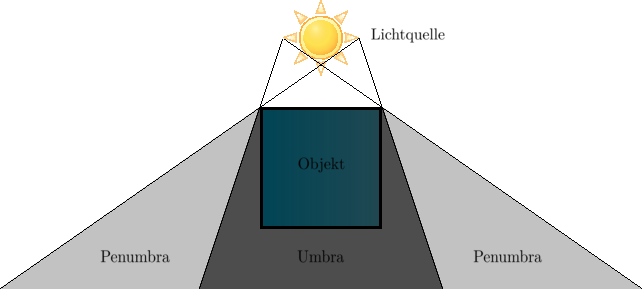
\includegraphics{img/shadowing.pdf}
    \caption{Illustration eines Schattenwurfes anhand einer Lichtquelle
        und einem Objekt. Im Bild sind die Umbra- und Penumbra-Regionen
        erkennbar.\protect\footnotemark}\label{fig:shadowing}
\end{figure}
\footnotetext{Eigene Darstellung mittels Inkscape, angelehnt
    an~\cite[S. 772]{glassner_introduction_1989}.}

\begin{lstlisting}[language=Python,caption={Algorithmus zur Berechnung
        von weichen Schatten.},label={alg:sphere_tracing_soft_shadows},captionpos=b,emph={calc_soft_shadows}]
def calc_soft_shadows():
    min_distance          = 0.01
    max_distance          = 9001
    shadow_ray_distance   = min_distance
    estimated_distance    = 0
    convergence_precision = 0.000001
    shadow                = 1.0
    scale                 = 32.0

    while shadow_ray_distance < max_distance:
        # sd_sphere is a signed distance function defining the implicit
        # surface, # cast_ray defines the ray equation given the current travelled /
        # marched distance of the ray
        estimated_distance = sd_sphere(cast_ray(shadow_ray_distance))

        if estimated_distance < convergence_precision:
            # the estimated distance is already smaller than the desired
            # precision of the convergence, so return zero (0) as we
            # have an intersection and therefore 'full' shadow
            return 0

        penumbra_factor = estimated_distance / shadow_ray_distance
        shadow = min(shadow, scale * penumbra_factor)
        shadow_ray_distance = shadow_ray_distance + estimated_distance

    # When we reach this point, there was no full intersection between
    # the ray and a implicit surface, so not entirely shadowed, so
    # return current shadow value
    return shadow
\end{lstlisting}



% -*- coding: UTF-8 -*-
% vim: autoindent expandtab tabstop=4 sw=4 sts=4 filetype=tex
% chktex-file 27 - disable warning about missing include files

\chapter{Diskussion und Fazit}
\label{chap:discussion_and_conclusion}

\section{Diskussion}
\label{sec:discussion}

\section{Erweiterungsmöglichkeiten}
\label{sec:further_work}

\section{Fazit}
\label{sec:fazit}


%---------------------------------------------------------------------------

% Glossary
%---------------------------------------------------------------------------
\cleardoublepage{}
\phantomsection{}
\addcontentsline{toc}{chapter}{Glossar}
\renewcommand{\glossaryname}{Glossar}
\glsaddall{}
\printglossaries{}
%---------------------------------------------------------------------------

% Bibliography
%---------------------------------------------------------------------------
%\cleardoublepage
\phantomsection{}
\addcontentsline{toc}{chapter}{Literaturverzeichnis}
\bibliographystyle{alpha}
\bibliography{inc/static/bibliography}{}
%---------------------------------------------------------------------------

% Listings
%---------------------------------------------------------------------------
%\cleardoublepage
\phantomsection{}
\addcontentsline{toc}{chapter}{Abbildungsverzeichnis}
\listoffigures
%\cleardoublepage
\phantomsection{}
\addcontentsline{toc}{chapter}{Tabellenverzeichnis}
\listoftables
%\cleardoublepage
\phantomsection{}
\addcontentsline{toc}{chapter}{Auflistungsverzeichnis}
\lstlistoflistings{}
%---------------------------------------------------------------------------

% Index
%---------------------------------------------------------------------------
%\cleardoublepage
%\phantomsection{}
%\addcontentsline{toc}{chapter}{Stichwortverzeichnis}
%\renewcommand{\indexname}{Stichwortverzeichnis}
%\printindex
%---------------------------------------------------------------------------

% Attachment:
%---------------------------------------------------------------------------
%\appendix
\settocdepth{section}
% -*- coding: UTF-8 -*-
% vim: autoindent expandtab tabstop=4 sw=4 sts=4 filetype=tex
% chktex-file 27

% In den Anhang fügen Sie ein:
%  * Details des Projektpans, falls vorhanden
%  * Resultate und Zwischenresultate in Funktion der Projektiterationen
%  * Pflichtenheft / Anforderungsspezifikation (Stand Ende dritter Woche)
%  * Angaben zum Projektrepository
%  * Sitzungsprotokolle, falls vorhanden
%  * Weiterführende Erläuterungen zu den verwendeten Technologien, falls nötig
%  * Benutzerhandbuch, falls vorhanden und sinnvoll, es hier aufzulisten
%  * Installations- und Betriebsdokument, falls vorhanden und sinnvoll, es hier aufzulisten
% Unterlassen Sie das Anfügen von Listings.

\appendix 
\begin{titlepage}
    \clearpage
    \vspace*{\fill}
    \begin{center}
        \begin{minipage}{.6\textwidth}
            \fontsize{26pt}{28pt}\selectfont
            \chapter*{Anhang}\label{chap:attachment}
            \addcontentsline{toc}{chapter}{Anhang}
        \end{minipage}
    \end{center}
    \vfill % equivalent to \vspace{\fill}
    \clearpage
\end{titlepage}

\newpage
 % -*- coding: UTF-8 -*-
% vim: autoindent expandtab tabstop=4 sw=4 sts=4 filetype=tex

\chapter{Meeting minutes}
\label{chap:10_meeting_minutes}

\VerbatimInput[label=20150921]{inc/static/attachment/minutes/20150921}



% \includepdfset{pagecommand={\thispagestyle{headings}}}
% \includepdf[pages=-, addtotoc={1,chapter,0,Anforderungsdokument,chap:anf},scale=0.95]{anhang/anforderungen.pdf}
% \newpage
% \includepdf[pages=-, addtotoc={1,chapter,0,Tutorial Wissensmodellierung,chap:tutorial},scale=0.95]{anhang/Tutorial.pdf}
% \newpage
% \input{anhang/schnipsel}
% \newpage
% \input{anhang/modellierung}
% \newpage
% \input{anhang/installationshandbuch}
% \newpage
% \includepdf[pages=-, addtotoc={1,chapter,0,Arbeitsjournal ,chap:arbeitsjournal},scale=0.95]{anhang/Journal.pdf}
% \newpage

%---------------------------------------------------------------------------

\end{document}
